\documentclass[12pt,a4paper]{report}
\usepackage[top=0.70in, bottom=0.70in, left=0.8in,right=0.80in]{geometry} % 
\usepackage[pdftex]{graphicx} %for embedding images
\usepackage[%dvips, % commented for pdflatex
bookmarks,  colorlinks=false]{hyperref}
\hypersetup{%
    pdfborder = {0 0 0}
}
\usepackage{verbatim}
\usepackage[final]{pdfpages} 
\usepackage{float}
\usepackage{hyperref}
\usepackage{pslatex}
\usepackage{array}
\usepackage{setspace}
\usepackage{float}
\usepackage{enumerate}
\usepackage{longtable}
\usepackage{multirow}
\usepackage[font=small,labelfont=bf]{caption}
\def\figurename{\textbf{Figure }}
\usepackage{fancyhdr}
\fancypagestyle{plain}{%
\fancyfoot[L]{\emph{Ingeniería de Software}} % except the center
\fancyfoot[R]{\thepage}
\renewcommand{\headrulewidth}{0.4pt}
\renewcommand{\footrulewidth}{0.4pt}
}
\pagestyle{fancy}
\rhead{\emph{Sistema de Administraci\'on Escolar}}
\fancyfoot[LO,LE]{\emph{Ingenier\'ia de Software}}
\cfoot{}
\fancyfoot[RO, RE]{\thepage}
\renewcommand{\headrulewidth}{0.4pt}
\renewcommand{\footrulewidth}{0.4pt}
\usepackage{pgf}
\usepackage{pgfpages}
\pgfpagesdeclarelayout{boxed}
{
  \edef\pgfpageoptionborder{0pt}
}
{
  \pgfpagesphysicalpageoptions
  {%
    logical pages=0,%
  }
  \pgfpageslogicalpageoptions{1}
  {
    border code=\pgfsetlinewidth{2pt}\pgfstroke,%
    border shrink=\pgfpageoptionborder,%
    resized width=.95\pgfphysicalwidth,%
    resized height=.95\pgfphysicalheight,%
    center=\pgfpoint{.5\pgfphysicalwidth}{.5\pgfphysicalheight}%
  }%
}
\pgfpagesuselayout{boxed}
\setlength{\parindent}{1cm}
\usepackage[utf8]{inputenc}
\usepackage[spanish]{babel} 

%%Cuadritos
\usepackage{enumitem,amssymb}
\newlist{checklist}{itemize}{2}
\setlist[checklist]{label=$\square$}
%%Cuadritos

\begin{document}
\tracingall
\renewcommand\bibname{Referencias Bibliográficas}
\lhead{ }

\newpage
\begin{center}
\thispagestyle{empty}
\LARGE{\textsc {\textbf{INSTITUTO POLITÉCNICO NACIONAL}}}\\[0.5cm]
\Large{\textbf{ESCUELA SUPERIOR DE CÓMPUTO}}\\[0.7cm]
\vspace{5cm}
\LARGE{\textbf{\\PLAN DE PRUEBAS\\}}
\vspace{7cm}
\end{center}
\Large{\textbf{\\INGENIERÍA DE SOFTWARE}}
\vspace{5cm}
\begin{flushright}
\Large{\textbf{\\30 de Octubre de 2017}}
\end{flushright}
\newpage
\newpage
\newpage
\begin{center}
\thispagestyle{empty}
\LARGE{\textsc {\textbf{INSTITUTO POLITÉCNICO NACIONAL}}}\\[0.5cm]
\Large{\textbf{ESCUELA SUPERIOR DE CÓMPUTO}}\\[0.7cm]
\vspace{0.5cm}
\Large{\textbf{\\PROYECTO}}
\LARGE{\textbf{\\``Sistema de Administración Escolar: SAES''\\}}
\vspace{2cm}
\Large{\textbf{\\INGENIERÍA DE SOFTWARE}}
\vspace{2cm}
\end{center}
\Large{\textbf{\\INTEGRANTES}}\\
\large{
\begin{itemize}
    \item BELTRÁN ALVARADO ROGELIO
    \item ESTRADA GRANADOS DIEGO
    \item HERNÁNDEZ PINEDA MIGUEL ANGEL
    \item HUITRÓN RIZO GABRIEL ALEJANDRO
    \item MATUS LÓPEZ CARLOS EDUARDO
    \item MEDINA LUQUEÑO ANA XIMENA
    \item MONROY MARTOS ELIOTH
    \item MONSALVO FUENTES AMÉRICA BERENICE
    \item OSORNIO DÍAZ EMILIANO
    \item PAREDES RIVAS ALBERTO
    \item TREJO GRANADOS YAHIR
\end{itemize}
}
\vspace*{1cm}
\large{\textbf{PROF. IDALIA CASTILLO MALDONADO}}\\
\newpage
\newpage
\pagenumbering{roman}
\pagestyle{empty}
\addtocontents{toc}{\protect\thispagestyle{empty}}
\tableofcontents
\cleardoublepage

\pagestyle{fancy}
\newpage
\pagenumbering{arabic}
\newpage
\chapter{Descripción de la Prueba}
\section{Propósito de la prueba}
\noindent
El presente documento tiene como objetivo la ejecución de las pruebas sobre el Sistema de Administración Escolar (en adelante SAES) con base en la especificación técnica.
\section{Alcance}
\noindent
Las pruebas que se presentan a continuación son pruebas unitarias de cada uno de los casos de uso del SAES.
\begin{itemize}
    \item Inicios de sesión en los diferentes perfiles.
    \item Registro de usuarios.
    \item Registro de materias.
    \item Registro de profesores.
    \item Registro de grupos.
    \item Generación de citas de inscripción.
    \item Reinscripción del alumno.
    \item Creación y almacenamiento de horarios.
    \item Edición de registros.
    \item Etcétera
\end{itemize}
\section{Elementos involucrados}
\noindent
Como se mencionó anteriormente se trabajará con todos los Casos de Uso que conforman el sistema, por lo tanto se verificarán todas las pantallas, así como los mensajes de alerta, confirmación y error que muestra el sistema. Los mensajes así como las pantallas del sistema se pueden encontrar en la sección de Anexos.
\section{Requerimientos}
\noindent
Las pruebas se ejecutarán en el laboratorio de la Escuela Superior de Cómputo haciendo uso de los equipos que se encuentran ahí. Es necesario tener las computadoras conectadas a una red local y que cada una de ellas tenga conexión con un equipo que será designado como el servidor. El navegador a ocupar será \textit{Google Chrome}.
\begin{longtable}{ | p{8cm} | p{7cm} | }
\hline
\multicolumn{2}{|p{15cm}|}{\textbf{Datos de Prueba}}\\
\hline
\textbf{Tipo de Prueba}: & Completa\\
\hline
\textbf{Fecha de Aplicación}: & \\
\hline
\textbf{Hora Inicio}: & \\
\hline
\textbf{Hora Final}: & \\
\hline
\textbf{Nombre del líder de pruebas}: & \\
\hline
\textbf{Nombre del tester}: & \\
\hline
\end{longtable}
\section{Checklist}
\noindent
Para poder dar inicio con las pruebas compruebe que cuenta con los siguientes puntos: \begin{itemize}
    \item Lápiz.
    \item Guión de Pruebas.
    \item El equipo cuenta con conexión al servidor.
    \item El equipo cuenta con el navegador Google Chrome.
\end{itemize}
\section{Instrucciones}
\begin{itemize}
    \item Verifique que cuenta con conexión al servidor de pruebas.
    \item Abra el navegador Google Chrome.
    \item Ingrese la siguiente dirección: 
\end{itemize}
\newpage
\chapter{Ejecución de Pruebas}
\section{Prueba P1: Caso de Uso Iniciar Sesión}
%Autor: Amé
\begin{longtable}{ | p{9cm} | p{.5cm} | p{.5cm} | p{5cm} | }
    \hline
    \textbf{Pregunta} 
    &
    \textbf{Si}
    &
    \textbf{No}
    &
    \textbf{Observaciones}\\
    \hline
    \multicolumn{4}{| p{15cm}| }{1. Seleccione ''Iniciar sesión” que se encuentra en la esquina superior derecha.
    }\\
	\hline
	1.1 ¿El Sistema lo dirigió a la pantalla 3.2 Iniciar Sesión?
	& & & \\
	\hline
	\multicolumn{4}{| p{15cm} |}{2. Oprima el botón ''Entrar''.
	}\\
	\hline
	2.1 ¿El Sistema evitó que iniciara sesión? 
	& & & \\
	\hline
	2.2 ¿El Sistema mostró mensaje de error ME.37?
	& & & \\
	\hline
	\multicolumn{4}{| p{15cm} |}{3. Ingrese el siguiente usuario:\newline\hspace{2cm}\textbf{MOFA970728H23}\newline4. Ingrese la siguiente contraseña:\newline\hspace{2cm}\textbf{Escom}\newline 5. Seleccione el botón ''Entrar''.
	}\\
	\hline
	5.1 ¿El Sistema mostró el mensaje de error ME.31?
	& & & \\
	\hline
	\multicolumn{4}{| p{15cm} |}{6. Vuelva a ingresar el usuario anterior, pero ahora ingrese como contraseña:\newline
	    \hspace{2cm}\textbf{Escom1234}\newline
	    7. Seleccione el botón ''Entrar''.
	}\\
	\hline
	7.1 ¿El Sistema le mostró el mensaje de error ME.32?
	& & & \\
	\hline
	\multicolumn{4}{| p{15cm} |}{8. Seleccione el botón ''Aceptar'' que muestra la ventana que contiene el mensaje.
	}\\
	\hline
	8.1 ¿El Sistema lo dirigió a la pantalla 3.2 Iniciar Sesión?
	& & & \\
	\hline
	\multicolumn{4}{| p{15cm} |}{9. Ingrese el siguiente usuario:\newline\hspace{2cm}\textbf{CAGM700215GS7}\newline10. Ingrese la siguiente contraseña:\newline\hspace{2cm}\textbf{Escom1234}\newline 11. Seleccione el botón ''Entrar''.
	}\\
	\hline
	11.1 ¿El Sistema lo dirigió a la pantalla 3.3 Datos Generales: Jefe de Gestión Escolar?\newline
	\textbf{Nota.-} El usuario es el Jefe de Gestión escolar.
	& & & \\
	\hline
	\multicolumn{4}{| p{15cm} |}{12. Verifique que se muestre en el apartado del lado derecho de la pantalla la siguiente información:
	    \textbf{Nombre: }María Guadalupe\newline
	    \textbf{Apellido Paterno: }Caro\newline
	    \textbf{Apellido Materno: }García\newline
	    \textbf{RFC: }CAGM700215GS7\newline
	    \textbf{Número de empleado: }2154146581\newline
	    \textbf{Correo: }sescolaresescom@ipn.mx}\\
	\hline
	12.1 ¿El Sistema mostró correctamente los datos anteriores (considere el mismo orden)? & & & \\
	\hline
	\multicolumn{4}{| p{15cm} |}{
	    \textbf{Fin de la Prueba}}\\
	\hline
\end{longtable}
\newpage
\section{Prueba P2: Caso de Uso Registrar alumno}
\begin{longtable}{ | p{9cm} | p{.5cm} | p{.5cm} | p{5cm} | }
\hline
\textbf{Pregunta} & \textbf{Si} & \textbf{No} & \textbf{Observaciones}\\
\hline
\multicolumn{4}{| p{15cm}| }{1. Acceda a la opción <<Registro>> del menú izquierdo y de clic en <<Registrar Alumno>>}\\
\hline
\multicolumn{4}{| p{15cm}| }{
		1.1. Evalúe la pantalla tomando como referencia 3.4 Registrar Alumno: Jefe de Gestión Escolar.
    \begin{checklist}
        \item Estilos CSS.
        \item Ortografía.
        \item Iconografía.
        \item Alineación.
    \end{checklist}}\\
\hline
\multicolumn{4}{| p{15cm}| }{2. Dé clic en el botón enviar sin ingresar datos.}\\
\hline
2.1 ¿El sistema evitó el registro del usuario? & & &\\
\hline
2.2 ¿El sistema mostró correctamente el error ME.37? & & &\\
\hline
\multicolumn{4}{| p{15cm}| }{3. Intente registrar un alumno con los siguientes datos: \begin{itemize}
    \item \textbf{Nombre:} Arturo
    \item \textbf{Apellido Paterno:} González
    \item \textbf{Apellido Materno:} Gómez
    \item \textbf{No. Boleta:} 2016630194
    \item \textbf{Correo Electrónico:} artgg@hotmail.com
    \item \textbf{Contraseña:} ARTgg2121
\end{itemize}} \\
\hline
3.1 ¿El sistema evitó el registro del usuario? & & &\\
\hline
3.2 ¿El sistema mostró correctamente el mensaje de error ME.3? & & &\\
\hline
\multicolumn{4}{| p{15cm}| }{4. Intente registrar un alumno con los siguientes datos: \begin{itemize}
    \item \textbf{Nombre:} Arturo
    \item \textbf{Apellido Paterno:} González
    \item \textbf{Apellido Materno:} Gómez
    \item \textbf{No. Boleta:} 2016631010
    \item \textbf{Correo Electrónico:} mirreyp@hotmail.com
    \item \textbf{Contraseña:} ARTgg2121
\end{itemize}} \\
\hline
4.1 ¿El sistema evitó el registro del usuario? & & &\\
\hline
4.2 ¿El sistema mostró correctamente el mensaje de error ME.2? & & &\\
\hline
\multicolumn{4}{| p{15cm}| }{5. Inicie el proceso de registrar un alumno con los siguientes datos: \begin{itemize}
    \item \textbf{Nombre:} Arturo
    \item \textbf{Apellido Paterno:} González
    \item \textbf{Apellido Materno:} Gómez
    \item \textbf{No. Boleta:} 2016631010
    \item \textbf{Correo Electrónico:} artgg@hotmail.com
    \item \textbf{Contraseña:} ARTgg2121
\end{itemize}} \\
\hline
5.1 ¿El sistema mostró el mensaje de confirmación MC.1? & & &\\
\hline
5.2 ¿El sistema redirigió la página a esta misma pantalla? & & &\\
\hline
\multicolumn{4}{| p{15cm}| }{\textbf{Fin de la Prueba}} \\
\hline
\end{longtable}
\newpage
\section{Prueba P3: Caso de Uso Registrar académico}
\begin{longtable}{ | p{9cm} | p{.5cm} | p{.5cm} | p{5cm} | }
\hline
\textbf{Pregunta} & \textbf{Si} & \textbf{No} & \textbf{Observaciones}\\
\hline
\multicolumn{4}{| p{15cm}| }{1. Acceda a la pantalla 3. Registrar Académico y de clic en el botón enviar sin ingresar datos.}\\
\hline
1.1 ¿El sistema evitó el registro del usuario? & & &\\
\hline
1.2 ¿El sistema mostró correctamente el error ME.1? & & &\\
\hline
\multicolumn{4}{| p{15cm}| }{2. Intente registrar un académico con el RFC \textbf{ABAJ8503330LK9}.} \\
\hline
2.1 ¿El sistema evitó el registro del usuario? & & &\\
\hline
2.2 ¿El sistema mostró correctamente el mensaje de error ME.4? & & &\\
\hline
\multicolumn{4}{| p{15cm}| }{3. Intente registrar un académico con el correo \textbf{abaj5@ipn.mx}.} \\
\hline
3.1 ¿El sistema evitó el registro del usuario? & & &\\
\hline
3.2 ¿El sistema mostró correctamente el mensaje de error ME.3? & & &\\
\hline
\multicolumn{4}{| p{15cm}| }{4. Intente registrar un académico ingresando datos que \textbf{no cumplan con el formato especificado} (repita el proceso en cada campo de dato)} \\
\hline
4.1 ¿El sistema evitó el registro del usuario? & & &\\
\hline
4.2 ¿El sistema mostró correctamente el mensaje de error ME.2? & & &\\
\hline
\multicolumn{4}{| p{15cm}| }{5. Inicie el proceso de registrar académico ingresando sus datos personales.} \\
\hline
5.1 ¿El sistema mostró el mensaje de confirmación MC.1? & & &\\
\hline
5.2 ¿El sistema redirigió la página a esta misma pantalla? & & &\\
\hline
\multicolumn{4}{| p{15cm}| }{\textbf{Fin de la Prueba}} \\
\hline
\end{longtable}
\newpage
\newpage
\section{Prueba P4: Caso de Uso Registrar analista}
\begin{longtable}{ | p{9cm} | p{.5cm} | p{.5cm} | p{5cm} | }
\hline
\textbf{Pregunta} & \textbf{Si} & \textbf{No} & \textbf{Observaciones}\\
\hline
\multicolumn{4}{| p{15cm}| }{1. Acceda a la opción <<Registro>> del menú izquierdo y de clic en la opción <<Registrar Analista>>}\\
\hline
\multicolumn{4}{| p{15cm}| }{
		1.1. Evalúe la pantalla tomando como referencia 3.5 Registrar Analista.
    \begin{checklist}
        \item Estilos CSS.
        \item Ortografía.
        \item Iconografía.
        \item Alineación.
    \end{checklist}}\\
\hline
\multicolumn{4}{| p{15cm}| }{2. Dé clic en el botón enviar sin ingresar datos.}\\
\hline
2.1 ¿El sistema evitó el registro del usuario? & & &\\
\hline
2.2 ¿El sistema mostró correctamente el error ME.37? & & &\\
\hline
\multicolumn{4}{| p{15cm}| }{3. Intente registrar un analista con los siguientes datos: \begin{itemize}
    \item \textbf{Nombre:} Miguel
    \item \textbf{Apellido Paterno:} Peña
    \item \textbf{Apellido Materno:} Gómez
    \item \textbf{Número de Empleado:} 2154146581
    \item \textbf{RFC:} PEGM770217HM7
    \item \textbf{Correo Electrónico:} pegom@hotmail.com
    \item \textbf{Contraseña:} ANpgm123
\end{itemize}} \\
\hline
3.1 ¿El sistema evitó el registro del usuario? & & &\\
\hline
3.2 ¿El sistema mostró correctamente el mensaje de error ME.4? & & &\\
\hline
\multicolumn{4}{| p{15cm}| }{4. Intente registrar un analista con los siguientes datos: \begin{itemize}
    \item \textbf{Nombre:} Miguel
    \item \textbf{Apellido Paterno:} Peña
    \item \textbf{Apellido Materno:} Gómez
    \item \textbf{Número de Empleado:} 2112344356
    \item \textbf{RFC:} PEVJ801210GF6
    \item \textbf{Correo Electrónico:} pegom@hotmail.com
    \item \textbf{Contraseña:} ANpgm123
\end{itemize}} \\
\hline
4.1 ¿El sistema evitó el registro del usuario? & & &\\
\hline
4.2 ¿El sistema mostró correctamente el mensaje de error ME.41? & & &\\
\hline
\multicolumn{4}{| p{15cm}| }{5. Intente registrar un analista con los siguientes datos: \begin{itemize}
    \item \textbf{Nombre:} Miguel
    \item \textbf{Apellido Paterno:} Peña
    \item \textbf{Apellido Materno:} Gómez
    \item \textbf{Número de Empleado:} 2112344356
    \item \textbf{RFC:} PEGM770217HM7
    \item \textbf{Correo Electrónico:} ferbotello@hotmail.com
    \item \textbf{Contraseña:} ANpgm123
\end{itemize}} \\
\hline
5.1 ¿El sistema evitó el registro del usuario? & & &\\
\hline
5.2 ¿El sistema mostró correctamente el mensaje de error ME.2? & & &\\
\hline
\multicolumn{4}{| p{15cm}| }{6. Inicie el proceso de registrar analista ingresando los siguientes datos (\textbf{X}):\begin{itemize}
    \item \textbf{Nombre:} Miguel
    \item \textbf{Apellido Paterno:} Peña
    \item \textbf{Apellido Materno:} Gómez
    \item \textbf{Número de Empleado:} 2112344356
    \item \textbf{RFC:} PEGM770217HM7
    \item \textbf{Correo Electrónico:} pegom@hotmail.com
    \item \textbf{Contraseña:} ANpgm123
\end{itemize}} \\
\hline
6.1 ¿El sistema mostró el mensaje de confirmación MC.1? & & &\\
\hline
6.2 ¿El sistema redirigió la página a esta misma pantalla? & & &\\
\hline
\multicolumn{4}{| p{15cm}| }{\textbf{Fin de la Prueba}} \\
\hline
\end{longtable}
\newpage
\section{Prueba P6: Caso de Uso Registrar materia}
\begin{longtable}{ | p{9cm} | p{.5cm} | p{.5cm} | p{5cm} | }
\hline
\textbf{Pregunta} & \textbf{Si} & \textbf{No} & \textbf{Observaciones}\\
\hline
\multicolumn{4}{| p{15cm}| }{1. Acceda a la opción <<Registro>> del menú izquierdo y de clic en la opción <<Registrar Grupo>>}\\
\hline
\multicolumn{4}{| p{15cm}| }{
		1.1. Evalúe la pantalla tomando como referencia 3.27 Registrar Materia.
    \begin{checklist}
        \item Estilos CSS.
        \item Ortografía.
        \item Iconografía.
        \item Alineación.
    \end{checklist}}\\
\hline
\multicolumn{4}{| p{15cm}| }{2. Dé clic en el botón enviar sin ingresar datos.}\\
\hline
2.1 ¿El sistema evitó el registro de la materia? & & &\\
\hline
2.2 ¿El sistema mostró correctamente el error ME.37? & & &\\
\hline
\multicolumn{4}{| p{15cm}| }{3. Inicie el proceso de registrar materia ingresando los siguientes datos (\textbf{X}):\begin{itemize}
    \item Nombre: Inteligencia Artificial
    \item Créditos: 4.39
    \item Nivel: 3
    \item Área: Formación Profesional
    \item Cupo: 25
\end{itemize}} \\
\hline
3.1 ¿El sistema mostró el mensaje de confirmación MC.1? & & &\\
\hline
3.2 ¿El sistema redirigió la página a esta misma pantalla? & & &\\
\hline
\multicolumn{4}{| p{15cm}| }{\textbf{Fin de la Prueba}} \\
\hline
\end{longtable}
\newpage
\section{Prueba P7: Caso de Uso Registrar profesor}
\begin{longtable}{ | p{9cm} | p{.5cm} | p{.5cm} | p{5cm} | }
\hline
\textbf{Pregunta} & \textbf{Si} & \textbf{No} & \textbf{Observaciones}\\
\hline
\multicolumn{4}{| p{15cm}| }{.De clic en el menú izquierdo en la opción <<Registro>>, posteriormente de clic en <<Registrar Profesor>>, cuando cargue la pantalla  de clic en el botón <<enviar>> sin ingresar datos.}\\
\hline
1.1 ¿El sistema evitó el registro del usuario? & & &\\
\hline
1.2 ¿El sistema mostró correctamente el error ME.1? & & &\\
\hline
\multicolumn{4}{| p{15cm}| }{2. Intente registrar un profesor con el RFC \textbf{OEGD7507074G7}.} \\
\hline
2.1 ¿El sistema evitó el registro del usuario? & & &\\
\hline
2.2 ¿El sistema mostró correctamente el mensaje de error ME.4? & & &\\
\hline
\multicolumn{4}{| p{15cm}| }{3. Intente registrar un profesor con el correo \textbf{didiog@gmail.com }.} \\
\hline
3.1 ¿El sistema evitó el registro del usuario? & & &\\
\hline
3.2 ¿El sistema mostró correctamente el mensaje de error ME.3? & & &\\
\hline
\multicolumn{4}{| p{15cm}| }{4. Intente registrar un profesor ingresando datos que \textbf{no cumplan con el formato especificado} (repita el proceso en cada campo de dato)} \\
\hline
4.1 ¿El sistema evitó el registro del usuario? & & &\\
\hline
4.2 ¿El sistema mostró correctamente el mensaje de error ME.2? & & &\\
\hline
\multicolumn{4}{| p{15cm}| }{5. Inicie el proceso de registrar profesor ingresando sus datos personales.} \\
\hline
5.1 ¿El sistema mostró el mensaje de confirmación MC.1? & & &\\
\hline
5.2 ¿El sistema redirigió la página a esta misma pantalla? & & &\\
\hline
\multicolumn{4}{| p{15cm}| }{\textbf{Fin de la Prueba}} \\
\hline
\end{longtable}
\newpage
\newpage
\section{Caso de Uso Generar Grupo}
\begin{longtable}{ | p{6cm} | p{10cm} |}
\hline
\textbf{NOMBRE} & Generar Grupo\\
\hline
\textbf{TIPO} & Primario\\
\hline
\textbf{DESCRIPCIÓN} & El analista registra los datos de un grupo nuevo en un formulario, asentándolo en el sistema.\\
\hline
\textbf{ENTRADAS} & Nivel: Selección de una lista numérica (entre 1 y 5)\\ & Turno: Selección de una lista (Matutino/Vespertino)\\ & Identificador: Entero Positivo\\
\hline
\textbf{SALIDAS} & Si el grupo fue dado de alta de forma exitosa se muestra un mensaje de confirmación.\\ & Si ocurrió algún error durante su registro, se muestra un mensaje con el error correspondiente.\\
\hline
\textbf{PRECONDICIONES} & El analista de gestión debe haber iniciado sesión.\\ & Es periodo de registro de grupos.\\
\hline
\textbf{POSTCONDICIONES} & El sistema se actualiza con los datos ingresados. Se muestra un mensaje de confirmación para avisar que el registro del grupo fue correcto.\\
\hline
\textbf{SITUACIONES DE ERROR} & \begin{itemize}
    \item El grupo ya ha sido registrado.
    \item Se dejaron campos obligatorios en blanco.
    \item El formato de los datos es inválido
\end{itemize}\\
\hline
\textbf{ESTADO DEL SISTEMA EN CASO DE ERROR} & El sistema no se actualiza.\\
\hline
\textbf{ACTORES} & Analista, Jefe de Gestión Escolar\\
\hline
\textbf{MENSAJES} & \textbf{Mensajes de Confirmación}: Se presentan en los siguientes casos: \begin{itemize}
    \item En caso de que se haya registrado exitosamente el nuevo grupo: MC.1.
\end{itemize}\\ & \textbf{Mensajes de Error}: Se presentan en los siguientes casos: \begin{itemize}
    \item El grupo ya ha sido registrado: ME.33
    \item Se dejaron campos obligatorios en blanco: ME.1
\end{itemize}\\
\hline
\textbf{AUTOR} & Medina Luqueño Ana Ximena\\
\hline
\end{longtable}
\vspace*{1cm}
\noindent
\Large{PROCEDIMIENTO ESTÁNDAR}
\large{}
\begin{enumerate}
    \item El usuario ingresa al sistema como analista de gestión escolar.
    \item El usuario selecciona la opción “Registrar grupo” en el menú de opciones.
    \item *El sistema carga el formulario para registrar grupos.
    \item El usuario selecciona el nivel y turno del grupo.
    \item El usuario ingresa el identificador del grupo.
    \item *El sistema valida que ninguno de los campos este vacío. \textbf{[Trayectoria 1]}
    \item *El sistema valida que los datos en el campo de identificador sean válidos. \textbf{[Trayectoria 2]}
    \item *El sistema valida que el grupo no haya sido registrado antes. \textbf{[Trayectoria 3]}
    \item *El sistema muestra el mensaje de confirmación correspondiente.
    \item *El sistema redirige a la pantalla de Registrar grupos.
    \item Fin del caso de uso.
\end{enumerate}
\vspace*{1cm}
\Large{PROCEDIMIENTOS ALTERNATIVOS}\\
\large{Trayectoria 1}\\
\textbf{Condición}: El usuario envió el formulario con algún campo vacío.
\begin{enumerate}
    \item *El sistema muestra el mensaje de error ME.1.
    \item Regresa al paso 4 de la trayectoria principal.
    \item Fin de la trayectoria.
\end{enumerate}
\large{Trayectoria 2}\\
\textbf{Condición}: Los datos en el campo de identificador son inválidos.
\begin{enumerate}
    \item *El sistema muestra el mensaje de error ME.2.
    \item Regresa al paso 5 de la trayectoria principal.
    \item Fin de la trayectoria.
\end{enumerate}
\large{Trayectoria 3}\\
\textbf{Condición}: El grupo ya ha sido registrado.
\begin{enumerate}
    \item *El sistema muestra el mensaje de error ME.33.
    \item Regresa al paso 4 de la trayectoria principal.
    \item Fin de la trayectoria.
\end{enumerate}
\newpage
\newpage
\section{Prueba P9: Caso de Uso Registrar grupo}
\begin{longtable}{ | p{9cm} | p{.5cm} | p{.5cm} | p{5cm} | }
\hline
\textbf{Pregunta} & \textbf{Si} & \textbf{No} & \textbf{Observaciones}\\
\hline
\multicolumn{4}{| p{15cm}| }{1. Acceda a la pantalla 3.9 Registrar grupo y de clic en el botón enviar sin ingresar datos.}\\
\hline
1.1 ¿El sistema evitó el registro del grupo? & & &\\
\hline
1.2 ¿El sistema mostró correctamente el error ME.1? & & &\\
\hline
\multicolumn{4}{| p{15cm}| }{2. Intente registrar un grupo ingresando los siguientes datos: \begin{itemize}
    \item Materia: Comunicación Oral y Escrita
    \item Profesor: Virginia Sánchez Cruz
    \item Grupo: 1CM1
    \item Horario: G
\end{itemize} } \\
\hline
2.1 ¿El sistema evitó el registro del grupo? & & &\\
\hline
2.2 ¿El sistema mostró correctamente el mensaje de error ME.14? & & &\\
\hline
\multicolumn{4}{| p{15cm}| }{3. Intente registrar un grupo ingresando los siguientes datos: \begin{itemize}
    \item Materia: Administración de Proyectos
    \item Profesor: Virginia Sánchez Cruz
    \item Grupo: 3CM2
    \item Horario: A
\end{itemize}}\\
\hline
3.1 ¿El sistema evitó el registro del grupo? & & &\\
\hline
3.2 ¿El sistema mostró correctamente el mensaje de error ME.15? & & &\\
\hline
\multicolumn{4}{| p{15cm}| }{4. Intente registrar un grupo ingresando los siguientes datos: \begin{itemize}
    \item Materia: Administración de Proyectos
    \item Profesor: Virginia Sánchez Cruz
    \item Grupo: 3CM2
    \item Horario: C
\end{itemize}} \\
\hline
4.1 ¿El sistema evitó el registro del grupo? & & &\\
\hline
4.2 ¿El sistema mostró correctamente el mensaje de error ME.16? & & &\\
\hline
    \multicolumn{4}{| p{15cm}| }{5. Inicie el proceso de registrar un grupo ingresando los siguientes datos (\textbf{X}): \begin{itemize}
    \item Materia: Liderazgo y Desarrollo Profesional
    \item Profesor: Virginia Sánchez Cruz
    \item Grupo: 3CM8
    \item Horario: C
\end{itemize} } \\
\hline
5.1 ¿El sistema mostró el mensaje de confirmación MC.1? & & &\\
\hline
5.2 ¿El sistema redirigió la página a esta misma pantalla? & & &\\
\hline
\multicolumn{4}{| p{15cm}| }{\textbf{Fin de la Prueba}} \\
\hline
\end{longtable}
\newpage
%Elioth Monroy El Chido
\section{Prueba P12: Caso de Uso Editar Profesor}
\begin{longtable}{ | p{9cm} | p{.5cm} | p{.5cm} | p{5cm} | }
	\hline
	\textbf{Pregunta} & \textbf{Si} & \textbf{No} & \textbf{Observaciones}\\
	\hline
	\multicolumn{4}{| p{15cm}| }{1. Inicie sesión en el sistema con los siguientes datos: \begin{itemize}
			\item Usuario: \textbf{CAGM700215GS7}
			\item Contraseña: \textbf{Escom1234}
		\end{itemize}
		2. En el menú izquierdo seleccione la opción <<Administrar>> y posteriormente de click en <<Profesor>>.}\\
		\hline
		2.1. ¿El sistema mostró la pantalla 3.15 Administrar Profesor? & & &\\
	\hline
	\multicolumn{4}{| p{15cm}| }{
		2.2. Evalúe la pantalla tomando como referencia 3.15 Administrar Profesor:
    \begin{checklist}
        \item Estilos CSS.
        \item Ortografía.
        \item Iconografía.
        \item Alineación.
    \end{checklist}}\\
	\hline
	\multicolumn{4}{| p{15cm}| }{
		3. En el campo <<Buscar>> ingrese el siguiente RFC: \textbf{AAFR720507EV8} y presione <<Buscar>>.\newline
		4. Posteriormente, al visualizar el resultado de la búsqueda, presione el botón <<Editar>>.}\\
		\hline
		4.1. ¿El sistema mostró la pantalla 3.16 Editar Profesor? & & &\\
	\hline
	\multicolumn{4}{| p{15cm}| }{
		4.2. Evalúe la pantalla tomando como referencia 3.16 Editar Profesor:
    \begin{checklist}
        \item Estilos CSS.
        \item Ortografía.
        \item Iconografía.
        \item Alineación.
    \end{checklist}}\\
	\hline
	\multicolumn{4}{| p{15cm}| }{	
		5. Llene el formulario con los siguientes datos y presione el botón <<Guardar>>: \begin{itemize}
			\item Nombre: Rocío 10
			\item Apellido paterno: Almazán
			\item Apellido materno: Farfán
			\item Número de empleado: 9823050566
			\item Correo electrónico: farfan@gmail.com
			\item Contraseña: Farfan1
	\end{itemize}}\\
	\hline
	5.1. ¿El sistema evitó que se guardaran los datos? & & &\\
	\hline
	5.2. ¿El sistema mostró correctamente el mensaje de error ME.38? & & &\\
	\hline
	\multicolumn{4}{| p{15cm}| }{6. Ingrese ahora los siguientes datos y presione <<Guardar>>:\begin{itemize}
			\item Nombre: Rocío 
			\item Apellido paterno: Almazán
			\item Apellido materno: Farfán
			\item Número de empleado: 9823050566
			\item Correo electrónico: maribel@gmail.com
			\item Contraseña: Farfan1
	\end{itemize}} \\
	\hline
	6.1. ¿El sistema evitó que se guardaran los datos? & & &\\
	\hline
	6.2. ¿El sistema mostró correctamente el mensaje de error ME.2? & & &\\
	\hline
	\multicolumn{4}{| p{15cm}| }{7. Ingrese ahora los siguientes datos y presione <<Guardar>>:\begin{itemize}
			\item Nombre: Rocío 
			\item Apellido paterno: Almazán
			\item Apellido materno: Farfán
			\item Número de empleado: 5324348509
			\item Correo electrónico: farfan@gmail.com
			\item Contraseña: Farfan1
	\end{itemize}} \\
	\hline
	7.1. ¿El sistema evitó que se guardaran los datos? & & &\\
	\hline
	7.2. ¿El sistema mostró correctamente el mensaje de error ME.4? & & &\\
	\hline
	\multicolumn{4}{| p{15cm}| }{8. Ingrese ahora los siguientes datos y presione <<Guardar>>:\begin{itemize}
			\item Nombre: Rocío
			\item Apellido paterno: Almazán
			\item Apellido materno: Farfán
			\item Número de empleado: 9823050566
			\item Correo electrónico: farfan@gmail.com
			\item Contraseña: Farfan2
	\end{itemize}} \\
	\hline
	8.1. ¿El sistema permitió que se guardaran los datos? & & &\\
	\hline
8.2. ¿El sistema mostró correctamente el mensaje de confirmación MC.3? & & &\\
	\hline
	\multicolumn{4}{| p{15cm}| }{\textbf{Fin de la Prueba}} \\
	\hline
\end{longtable}
\newpage
\begin{comment}
\newpage
\section{Caso de Uso Editar Académico}
\begin{longtable}{ | p{6cm} | p{10cm} |}
    \hline
    \textbf{NOMBRE} & Editar Académico\\
    \hline
    \textbf{TIPO} & Primario\\
    \hline
    \textbf{DESCRIPCIÓN} & El jefe de gestión escolar o un analista modifica los datos de un académico registrado en el sistema.\\
    \hline
    \textbf{ENTRADAS} &
    \begin{itemize}
    	\item Nombre del Académico: Caracteres (solo letras).
    	\item Apellido Paterno: Caracteres (solo letras).
    	\item Apellido Materno: Caracteres (solo letras).
    	\item Número de empleado: Número con longitud de 10 dígitos.
    	\item Correo Electrónico: Caracteres con el formato de correo electrónico.
    	\item Contraseña: Cadena con una longitud de 6 a 20 caracteres.
    \end{itemize}\\  
    \hline
    \textbf{SALIDAS} & Mensaje de éxito o mensaje de error según sea el caso.\\
    \hline
    \textbf{PRECONDICIONES} & El académico a editar debe estar previamente registrado.\\
    \hline
    \textbf{POSTCONDICIONES} & Se registran los nuevos datos del Académico en la base de datos.\\
    \hline
    \textbf{SITUACIONES DE ERROR} &Se presentan en los siguientes casos:
    \begin{itemize}
    	\item Se dejaron campos obligatorios en blanco.
    	\item El correo ya ha sido registrado en otra cuenta.
    	\item El formato de los datos es inválido.
    	\item El número de empleado ya fue asignado a otro Académico.
    \end{itemize}\\
    \hline
    \textbf{ESTADO DEL SISTEMA EN CASO DE ERROR} &  En espera de nuevas entradas.\\
    \hline
    \textbf{ACTORES} & Jefe de Gestión Escolar, Analista\\
    \hline
    \textbf{MENSAJES}  & \textbf{Mensaje de Confirmación}: Se muestra cuando los datos han sido almacenados correctamente: MC.3\\&\textbf{Mensajes de Error}: Se muestran en los siguientes casos:\begin{itemize}
    	\item Se dejaron campos obligatorios en blanco: ME.37
    	\item El formato de los datos es inválido: ME.31, ME.38, ME.39, ME.40
    	\item El correo está registrado en otra cuenta: ME.2
    	\item El número de empleado ya fue asignado a otro Académico: ME.4
    \end{itemize}\\
    \hline
    \textbf{AUTOR} & Monroy Martos Elioth\\
    \hline
\end{longtable}
\vspace*{1cm}
\noindent
\Large{PROCEDIMIENTO ESTÁNDAR}
\large{}
\begin{enumerate}
	\item El usuario ingresa al sistema como Jefe de Gestión Escolar o Analista.
	\item El usuario da click en la opción de <<Administrar Académico>> de la sección <<Administrar>>.
	\item El usuario ingresa el RFC del académico a modificar y presiona el botón <<Buscar>> (Figura 3.13).
	\textbf{[Trayectoria 1]}
	\item *El sistema le muestra al usuario los resultados obtenidos de su búsqueda en forma de lista.
	\item El usuario presiona el botón <<Editar>> del académico que desea editar (Figura 3.14).
	\item *El sistema le muestra el formulario de edición de académico al usuario.
	\item El usuario ingresa la nueva información del académico.
	\item El usuario da click en el botón <<Guardar>>.
	\item El sistema valida que no haya campos obligatorios en blanco. \textbf{[Trayectoria 2]}
	\item *El sistema valida los datos en el campo de nombre. \textbf{[Trayectoria 3]}
	\item *El sistema valida los datos en el campo de apellido paterno. \textbf{[Trayectoria 4]}
	\item *El sistema valida los datos en el campo de apellido materno. \textbf{[Trayectoria 5]}
	\item *El sistema valida los datos en el campo de número de empleado. \textbf{[Trayectoria 6]} \textbf{[Trayectoria 9]}
	\item *El sistema valida los datos en el campo de correo electrónico. \textbf{[Trayectoria 7]}
	\item *El sistema valida los datos en el campo de contraseña según la regla de negocio RN.2. \textbf{[Trayectoria 8]}
	\item *El sistema almacena los nuevos datos del académico y reemplaza los anteriores.
	\item *El sistema muestra el mensaje de confirmación MC.3.
	\item Fin del caso de uso.
\end{enumerate}
\vspace*{1cm}
\Large{PROCEDIMIENTOS ALTERNATIVOS}\\
\large{Trayectoria 1}\\
\textbf{Condición}: La búsqueda de académicos no obtuvo resultados.
\begin{enumerate}
	\item *El sistema muestra el mensaje de error ME.23.
	\item Regresa al punto 3 de la trayectoria principal.
	\item Fin de la trayectoria.
\end{enumerate}
\large{Trayectoria 2}\\
\textbf{Condición}: Quedaron campos obligatorios en blanco.
\begin{enumerate}
	\item *El sistema muestra el mensaje de error ME.37.
	\item *El sistema marca el campo vacío.
	\item Regresa al punto 3 de la trayectoria principal.
	\item Fin de la trayectoria.
\end{enumerate}
\large{Trayectoria 3}\\
\textbf{Condición}: El formato de texto para el campo <<Nombre>> es inválido.
\begin{enumerate}
	\item *El sistema muestra el mensaje de error ME.38.
	\item *El sistema marca el campo <<Nombre>>.
	\item Regresa al punto 7 de la trayectoria principal.
	\item Fin de la trayectoria.
\end{enumerate}
\large{Trayectoria 4}\\
\textbf{Condición}: El formato de texto para el campo <<Apellido Paterno>> es inválido.
\begin{enumerate}
	\item *El sistema muestra el mensaje de error ME.38.
	\item *El sistema marca el campo <<Apellido Paterno>>.
	\item Regresa al punto 7 de la trayectoria principal.
	\item Fin de la trayectoria.
\end{enumerate}
\large{Trayectoria 5}\\
\textbf{Condición}: El formato de texto para el campo <<Apellido Materno>> es inválido.
\begin{enumerate}
	\item *El sistema muestra el mensaje de error ME.38.
	\item *El sistema marca el campo <<Apellido Materno>>.
	\item Regresa al punto 7 de la trayectoria principal.
	\item Fin de la trayectoria.
\end{enumerate}
\large{Trayectoria 6}\\
\textbf{Condición}: El formato de los datos en el campo <<Número de Empleado>> es inválido.
\begin{enumerate}
	\item *El sistema muestra el mensaje de error ME.38.
	\item *El sistema marca el campo <<Número de Empleado>>.
	\item Regresa al punto 7 de la trayectoria principal.
	\item Fin de la trayectoria.
\end{enumerate}
\large{Trayectoria 7}\\
\textbf{Condición}: El formato del correo electrónico es inválido.
\begin{enumerate}
	\item *El sistema muestra alguno de los mensajes de error: ME.39, ME.40.
	\item *El sistema marca el campo <<Correo Electrónico>>.
	\item Regresa al punto 7 de la trayectoria principal.
	\item Fin de la trayectoria.
\end{enumerate}
\large{Trayectoria 8}\\
\textbf{Condición}: El formato de la contraseña es inválido según la regla de negocio RN.2.
\begin{enumerate}
	\item *El sistema muestra alguno de los mensajes de error: ME.31, ME.38.
	\item *El sistema marca el campo <<Contraseña>>.
	\item Regresa al punto 7 de la trayectoria principal.
	\item Fin de la trayectoria.
\end{enumerate}
\large{Trayectoria 9}\\
\textbf{Condición}: El número de empleado asignado ya ha sido registrado.
\begin{enumerate}
	\item *El sistema muestra el mensaje de error ME.4.
	\item *El sistema marca el campo <<Número de Empleado>>.
	\item Regresa al punto 7 de la trayectoria principal.
	\item Fin de la trayectoria.
\end{enumerate}
\newpage
\section{Prueba P14: Caso de Uso Editar Grupo}
\begin{longtable}{ | p{9cm} | p{.5cm} | p{.5cm} | p{5cm} | }
	\hline
	\textbf{Pregunta} & \textbf{Si} & \textbf{No} & \textbf{Observaciones}\\
	\hline
	\multicolumn{4}{| p{15cm}| }{1. Inicie sesión en el sistema con los siguientes datos: \begin{itemize}
			\item Usuario: \textbf{CAGM700215GS7}
			\item Contraseña: \textbf{Oscar1}
		\end{itemize}
		2. En el menú izquierdo seleccione la opción <<Administrar>> y posteriormente de click en <<Grupo>>.\newline
		3. En el campo <<Buscar>> ingrese el siguiente numero: 4 y presione <<Buscar>>.\newline
		4. Posteriormente, al visualizar el resultado de la búsqueda,seleccione el grupo numero 1, presione el botón <<Editar>>.
	}\\
	\hline
	\multicolumn{4}{| p{15cm}| }{2. Ingrese ahora los siguientes datos y presione <<Guardar>>:\begin{itemize}
			\item Turno: Vespertino
			\item Nivel: 4
			\item Numero del grupo: 1
	\end{itemize}} \\
	\hline
	2.1 ¿El sistema evitó que se guardaran los datos? & & &\\
	\hline
	2.2 ¿El sistema mostró correctamente el mensaje de error ME.3? & & &\\
	\hline
\multicolumn{4}{| p{15cm}| }{3. Ingrese ahora los siguientes datos y presione <<Guardar>>:
    \begin{itemize}
			\item Turno: Matutino
			\item Nivel: 3
			\item Numero del grupo: 1
	\end{itemize} 
	}\\
	\hline
	3.1 ¿El sistema evitó que se guardaran los datos? & & &\\
	\hline
	3.2 ¿El sistema mostró correctamente el mensaje de error ME.5? & & &\\
	\hline
	\multicolumn{4}{| p{15cm}| }{4. Ingrese ahora los siguientes datos y presione <<Guardar>>:\begin{itemize}
			\item Turno: Matutino
			\item Nivel: 4
			\item Numero del grupo: 15
	\end{itemize}} \\
	\hline
	4.1 ¿El sistema permitió que se guardaran los datos? & & &\\
	\hline
	4.2 ¿El sistema mostró correctamente el mensaje de confirmación MC.1? & & &\\
	\hline
	\multicolumn{4}{| p{15cm}| }{\textbf{Fin de la Prueba}} \\
	\hline
\end{longtable}
\newpage
\section{Prueba P15: Caso de Uso Editar Materia}
\begin{longtable}{ | p{9cm} | p{.5cm} | p{.5cm} | p{5cm} | }
	\hline
	\textbf{Pregunta} & \textbf{Si} & \textbf{No} & \textbf{Observaciones}\\
	\hline
	\multicolumn{4}{| p{15cm}| }{1. Inicie sesión en el sistema con los siguientes datos: \begin{itemize}
			\item Usuario: \textbf{GUMO7702172S8}
			\item Contraseña: \textbf{Oscar1}
		\end{itemize}
		2. En el menú izquierdo seleccione la opción <<Administrar>> y posteriormente de click en <<Materia>>.\newline
		3. En el campo <<Buscar>> ingrese el siguiente nombre: \textbf{Redes de computadoras} y presione <<Buscar>>.\newline
		4. Posteriormente, al visualizar el resultado de la búsqueda, presione el botón <<Editar>>.\newline
		5. En la pantalla 3.18 Administrar Materia, llene el formulario con datos inválidos y presione el botón <<Guardar>>}\\
	\hline
	5.1 ¿El sistema evitó que se guardaran los datos? & & &\\
	\hline
	5.2 ¿El sistema mostró correctamente el mensaje de error ME.2? & & &\\
	\hline
	\multicolumn{4}{| p{15cm}| }{6. Ingrese ahora los siguientes datos y presione <<Guardar>>:\begin{itemize}
			\item Nombre: Redes de las computadoras 
			\item Nivel: 2
			\item Créditos: 14
			\item Clasificación: Formación profesional
	\end{itemize}} \\
	\hline
	6.1 ¿El sistema evitó que se guardaran los datos? & & &\\
	\hline
	6.2 ¿El sistema mostró correctamente el mensaje de error ME.3? & & &\\
	\hline
	\multicolumn{4}{| p{15cm}| }{7. Ingrese ahora los siguientes datos y presione <<Guardar>>:\begin{itemize}
			\item Nombre: Redes de las computadoras 
			\item Nivel: 2
			\item Créditos: 5
			\item Clasificación: Formación profesional
	\end{itemize}} \\
	\hline
	7.1 ¿El sistema permitió que se guardaran los datos? & & &\\
	\hline
	7.2 ¿El sistema mostró correctamente el mensaje de confirmación MC.1? & & &\\
	\hline
	\multicolumn{4}{| p{15cm}| }{\textbf{Fin de la Prueba}} \\
	\hline
\end{longtable}
\newpage
\newpage
\section{Prueba P16: Caso de Uso Restablecer Contraseña}
\begin{longtable}{ | p{9cm} | p{.5cm} | p{.5cm} | p{5cm} | }
\hline
\textbf{Pregunta} & \textbf{Si} & \textbf{No} & \textbf{Observaciones}\\
\hline
\multicolumn{4}{| p{15cm}| }{1. Seleccione la opción <<Iniciar Sesión>> de la pantalla de Inicio.\newline 2. Seleccione la opción <<Restablecer Contraseña>> del formulario de inicio de sesión. \newline 3. Envíe el formulario desplegado sin ingresar datos dándole clic en Enviar.
}\\
\hline
3.1  ¿El sistema mostró correctamente el ME.1? & & &\\
3.2  ¿El sistema redirigió a la pantalla de Restablecer Contraseña? & & &\\
\hline
\textbf{Pregunta} & \textbf{Si} & \textbf{No} & \textbf{Observaciones}\\
\hline
\multicolumn{4}{| p{15cm}| }{4. Ingrese ahora el usuario \textbf{2016630199} y envíe el formulario dándole clic en Enviar.}\\
\hline
4.1  ¿El sistema mostró correctamente el ME.6? & & &\\
\hline
\textbf{Pregunta} & \textbf{Si} & \textbf{No} & \textbf{Observaciones}\\
\hline
\multicolumn{4}{| p{15cm}| }{5. Ingrese ahora el usuario \textbf{2016630194} y envíe el formulario dándole clic en Enviar.}\\
\hline
5.1  ¿El sistema mostró correctamente la ME.2? & & &\\
\hline
\multicolumn{4}{| p{15cm}| }{\textbf{Fin de la Prueba}} \\
\hline
\end{longtable}
\newpage
\newpage
\section{Prueba P17: Caso de Uso Cambiar Contraseña}
\begin{longtable}{ | p{9cm} | p{.5cm} | p{.5cm} | p{5cm} | }
\hline
\textbf{Pregunta} & \textbf{Si} & \textbf{No} & \textbf{Observaciones}\\
\hline
\multicolumn{4}{| p{15cm}| }{1. Inicie sesión en el sistema con los siguientes datos: \begin{itemize}
    \item Usuario: \textbf{2016630521}
    \item Contraseña: \textbf{Trejo1}
\end{itemize}
2. En el menú desplegable derecho seleccione la opción <<Cambiar Contraseña>>.}\\
\hline
    2.1 ¿El sistema mostró la pantalla 3.20 Cambiar Contraseña? & & &\\
\hline
\multicolumn{4}{| p{15cm}| }{
		2.2. Evalúe la pantalla tomando como referencia Cambiar Contraseña:
    \begin{checklist}
        \item Estilos CSS.
        \item Ortografía.
        \item Iconografía.
        \item Alineación.
    \end{checklist}}\\
\hline
\multicolumn{4}{| p{15cm}| }{
    3. En la pantalla 3.2 Cambiar Contraseña, envíe el formulario con los campos vacíos dando clic en Enviar.}\\
\hline
    3.1 ¿El sistema evitó el cambio de contraseña del usuario? & & &\\
\hline
    3.2 ¿El sistema mostró correctamente el error ME.37 al primer campo del formulario? & & &\\
\hline
\multicolumn{4}{| p{15cm}| }{4. Intente cambiar la contraseña ingresando los siguientes datos y luego mandando el formulario dando clic en enviar: \begin{itemize}
    \item Contraseña actual: \textbf{Trejo2}
	\item Nueva contraseña: \textbf{NuevaContrasena1}
	\item Confirmar contraseña: \textbf{NuevaContrasena1}
\end{itemize}} \\
\hline
    4.1 ¿El sistema evitó la actualización de la contraseña? & & &\\
\hline
    4.2 ¿El sistema mostró correctamente el mensaje de error ME.42? & & &\\
\hline
\multicolumn{4}{| p{15cm}| }{5. Intente cambiar la contraseña ingresando los siguientes datos y luego mandando el formulario dando clic en enviar: \begin{itemize}
    \item Contraseña actual: \textbf{Trejo1}
	\item Nueva contraseña: \textbf{NuevaContrasena1}
	\item Confirmar contraseña: \textbf{NuevaContrasena2}
\end{itemize}} \\
\hline
    5.1 ¿El sistema evitó la actualización de la contraseña? & & &\\
\hline
    5.2 ¿El sistema mostró correctamente el mensaje de error ME.43? & & &\\
\hline
\multicolumn{4}{| p{15cm}| }{6. Intente cambiar la contraseña ingresando los siguientes datos y luego mandando el formulario dando clic en enviar: \begin{itemize}
    \item Contraseña actual: \textbf{Trejo1}
	\item Nueva contraseña: \textbf{NuevaContrasena1}
	\item Confirmar contraseña: \textbf{NuevaContrasena1}
\end{itemize}} \\
\hline
    6.1 ¿El sistema mostró el mensaje de confirmación MC.3? & & &\\
\hline
    6.2 ¿El sistema lo redirigió al formulario de inicio de sesión pantalla 3.2 Login? & & &\\
\hline
\multicolumn{4}{| p{15cm}| }{\textbf{Fin de la Prueba}} \\
\hline
\end{longtable}
\newpage
\section{Prueba P18: Caso de Uso Ver Alumno}
\begin{longtable}{ | p{9cm} | p{.5cm} | p{.5cm} | p{5cm} | }
\hline
\textbf{Pregunta} & \textbf{Si} & \textbf{No} & \textbf{Observaciones}\\
\hline
\multicolumn{4}{| p{15cm}| }{1. Acceda a la pantalla 3.18 Ver Alumno e ingrese el número de boleta \textbf{2016630000}}\\
\hline
1.1 ¿El sistema mostró correctamente el error ME.18? & & &\\
\hline
\multicolumn{4}{| p{15cm}| }{2. Ingrese el número de boleta \textbf{2016630194}} \\
\hline
2.1 ¿El sistema muestra los datos del alumno correctamente? & & &\\
\hline
2.2 ¿Se muestran el botón reinscribir? & & &\\
\hline
2.3 ¿Se muestran el botón dar de baja? & & &\\
\hline
\multicolumn{4}{| p{15cm}| }{\textbf{Fin de la Prueba}} \\
\hline
\end{longtable}
\newpage
\newpage
\section{Caso de Uso Habilitar Reinscripción}
\begin{longtable}{ | p{6cm} | p{10cm} |}
    \hline
    \textbf{NOMBRE} & Habilitar Reinscripción\\
    \hline
    \textbf{TIPO} & Primario\\
    \hline
    \textbf{DESCRIPCIÓN} & El jefe de gestión escolar, selecciona dos fechas, inicio y fin del periodo de reinscripciones respectivamente, lo cual da como resultado que sea habilitado el período de reinscripciones en el sistema.\\
    \hline
    \textbf{ENTRADAS} & Fecha de inicio del período de reinscripciones y fecha de término.\\&Hora de inicio y fin de las inscripciones\\
    \hline
    \textbf{SALIDAS} & Mensaje de éxito o mensaje de error dependiendo del caso.\\
    \hline
    \textbf{PRECONDICIONES} & El usuario debe ser autenticado como Jefe de Gestión Escolar y no debe de estar habilitado ningún otro periodo de reinscripciones.\\
    \hline
    \textbf{POSTCONDICIONES} & El sistema crea las citas de reinscripción para todos los estudiantes inscritos automáticamente y notifica al usuario en caso de que haya existido un error, de igual manera notifica al usuario en el caso de que todas las citas de reinscripción hayan sido creadas satisfactoriamente.\\
    \hline
    \textbf{SITUACIONES DE ERROR} &Se presenta un error en las siguientes situaciones:
    \begin{itemize}
        \item No todos los campos del formulario fueron llenados.
    	\item No todos los alumnos inscritos obtienen una cita de reinscripción.
    	\item Las fecha de término del periodo de reinscripciones no es posterior a la fecha de inicio.
    	\item La hora de finalización por día del periodo de reinscripciones no es posterior a la hora de inicio.
    	\item El periodo de reinscripciones seleccionado es menor a tres días.
    \end{itemize}\\
    \hline
    \textbf{ESTADO DEL SISTEMA EN CASO DE ERROR} &  En espera de que el Jefe de Gestión Escolar asigne una cita de reinscripción a los alumnos faltantes.\\
    \hline
    \textbf{ACTORES} & Jefe de Gestión Escolar\\
    \hline
    \textbf{MENSAJES} & \textbf{Mensaje de confirmación}: Se presenta cuando todos los alumnos inscritos obtienen una cita de inscripción: MC.4.\\&\textbf{Mensaje de error}: Se presentan en los siguientes casos:
    \begin{itemize}
    \item Cuando al menos uno de los campos del formulario no fue llenado: ME.37
\item Cuando al menos uno de los estudiantes inscritos no obtuvo una cita de reinscripción: ME.13
\item Cuando la fecha de término del periodo de reinscripción no es posterior a la fecha de inicio: ME.26
\item Cuando la hora de finalización por día del periodo de reinscripciones no es posterior a la hora de inicio: ME.27
\item Cuando el periodo seleccionado para reinscripciones tiene una duración menor a tres días: ME.28
\end{itemize}\\
    \hline
    \textbf{AUTOR} & Monroy Martos Elioth\\
    \hline
\end{longtable}
\vspace*{1cm}
\noindent
\Large{PROCEDIMIENTO ESTÁNDAR}
\large{}
\begin{enumerate}
    \item El usuario accede al sistema como Jefe de Gestión Escolar.
	\item El Jefe de Gestión Escolar da click en la opción <<Períodos>> dentro de la sección Administrar.
	\item El Jefe de Gestión Escolar selecciona el período de inicio de las reinscripciones al presionar el campo <<Inicio>>, posteriormente selecciona la fecha de término de las reinscripciones al presionar el campo <<Final>> (Figura 3.19).
	\item El Jefe de Gestión Escolar presiona el botón <<Enviar>>
	\item *El sistema valida que la fecha de término sea posterior a la fecha de inicio.\\$\left[\textbf{Trayectoria 1}\right]$
	$\left[\textbf{Trayectoria 2}\right]$
	$\left[\textbf{Trayectoria 3}\right]$
	\item *El sistema genera las citas de reinscripciones correspondientes para todos los alumnos inscritos.$\left[\textbf{Trayectoria 4}\right]$
	\item *El sistema muestra el mensaje de confirmación MC.4.
	\item Fin de caso de uso.
\end{enumerate}
\vspace*{1cm}
\Large{PROCEDIMIENTOS ALTERNATIVOS}\\
\large{Trayectoria 1}\\
\textbf{Condición}: Las fecha u hora de término no es posterior a la fecha u hora de inicio de las reinscripciones.
\begin{enumerate}
		\item *El sistema muestra el mensaje de error ME.26 o ME.27.
		\item *Se vuelve al punto 3 de la trayectoria Principal.
		\item Fin de trayectoria.
\end{enumerate}
\large{Trayectoria 2}\\
\textbf{Condición}: La duración del periodo de reinscripciones es menor a tres días.
\begin{enumerate}
		\item *El sistema muestra el mensaje de error ME.28.
		\item *Se vuelve al punto 3 de la trayectoria Principal.
		\item Fin de trayectoria.
\end{enumerate}
\large{Trayectoria 3}\\
\textbf{Condición}: Al menos uno de los campos del formulario no fue llenado.
\begin{enumerate}
		\item *El sistema muestra el mensaje de error ME.37.
		\item *El sistema señala el primer campo que no haya sido llenado.
		\item *Se vuelve al punto 3 de la trayectoria Principal.
		\item Fin de trayectoria.
\end{enumerate}
\large{Trayectoria 4}\\
\textbf{Condición}: No todos los alumnos inscritos obtuvieron una cita de reinscripción.
\begin{enumerate}
		\item *El sistema muestra el mensaje de error ME.13 al usuario y le muestra un botón llamado <<Asignar Citas Manualmente>>.
		\item El Jefe de Departamento presiona el botón <<Asignar Citas Manualmente>>.
		\item *El sistema inicia el caso de uso <<Asignar Citas Manualmente>>.
		\item Fin de trayectoria.
\end{enumerate}
\newpage
\section{Prueba P20: Caso de Buscar Materia}
\begin{longtable}{ | p{9cm} | p{.5cm} | p{.5cm} | p{5cm} | }
	\hline
	\textbf{Pregunta} & \textbf{Si} & \textbf{No} & \textbf{Observaciones}\\
	\hline
	\multicolumn{4}{| p{15cm}| }{1. Inicie sesión en el sistema con los siguientes datos: \begin{itemize}
			\item Usuario: \textbf{2016630001}
			\item Contraseña: \textbf{Emiliano1}
		\end{itemize}
		2. En el menú izquierdo seleccione la opción <<Reinscripción>> y posteriormente de clic en <<Crear Horario>>.\newline
		3. En el campo <<Buscar>> déjelo en blanco y presione enter.}\\
	\hline
	1.1 ¿El sistema muestra materias?& & &\\
	\multicolumn{4}{| p{15cm}| }{2. Ingrese ahora "Cálculo" y presione Enter}\\
	\hline
	2.1 ¿El sistema muestra materias?& & &\\
	\hline
	\multicolumn{4}{| p{15cm}| }{3. Ingrese ahora "1CM10" y presione Enter}\\
	\hline
	3.1 ¿El sistema muestra materias?& & &\\
	\hline
	\multicolumn{4}{| p{15cm}| }{4. Ingrese ahora "Luna" y presione Enter}\\
	\hline
	4.1 ¿El sistema muestra materias?& & &\\
	\hline
	\multicolumn{4}{| p{15cm}| }{5. Ingrese ahora "Héctor Rojas Luna" y presione Enter}\\
	\hline
	5.1 ¿El sistema muestra materias?& & &\\
	\hline
	\multicolumn{4}{| p{15cm}| }{6. Ingrese ahora "1CM11" y presione Enter}\\
	\hline
	6.1 ¿El sistema muestra materias?& & &\\
	\hline
\end{longtable}
\newpage
%Elioth Monroy El Chido
\section{Prueba P21: Caso de Uso Crear Horario}
\begin{longtable}{ | p{9cm} | p{.5cm} | p{.5cm} | p{5cm} | }
\hline
\textbf{Pregunta} & \textbf{Si} & \textbf{No} & \textbf{Observaciones}\\
\hline
\multicolumn{4}{| p{15cm}| }{1. Inicie sesión en el sistema con los siguientes datos: \begin{itemize}
		\item Usuario: \textbf{2015631008}
		\item Contraseña: \textbf{Juanito1}
	\end{itemize}
	 2. En el menú izquierdo seleccione la opción <<Reinscripción>> y posteriormente de click en <<Crear horario>>.}\\
	 \hline
	 2.1. ¿El sistema mostró la pantalla 3.49 Crear Horario 1? & & &\\
	\hline
	\multicolumn{4}{| p{15cm}| }{
	2.2. Evalúe la pantalla tomando como referencia 3.49 Crear Horario 1:
    \begin{checklist}
        \item Estilos CSS.
        \item Ortografía.
        \item Iconografía.
        \item Alineación.
    \end{checklist}}\\
	\hline
	 \multicolumn{4}{| p{15cm}| }{
	 3. En el campo <<Buscar materias>> ingrese el siguiente valor: \textbf{1CM10}, presionar el botón <<Agregar>> para la materia de <<Cálculo>>.}\\
\hline
3.1. ¿El sistema mostró correctamente el mensaje de error ME.15? & & &\\
\hline
3.2. ¿El sistema evitó que la materia fuera agregada al horario? & & &\\
\hline
\multicolumn{4}{| p{15cm}| }{4. Busque el grupo <<1CM1>> y agregue la materia de <<Física>>.\newline Posteriormente, busque el grupo <<1CM2>> y agregue la materia de <<Cálculo>>}\\
\hline
4.1. ¿El sistema mostró correctamente el mensaje de error ME.16? & & &\\
\hline
4.2. ¿El sistema evitó que la materia fuera agregada al horario? & & &\\
\hline
\multicolumn{4}{| p{15cm}| }{5. Busque el grupo <<1CM2>> y agregue la materia de <<Física>>}\\
\hline
5.1 ¿El sistema mostró correctamente el mensaje de error ME.17? & & &\\
\hline
5.2 ¿El sistema evitó que la materia fuera agregada al horario? & & &\\
\hline
\multicolumn{4}{| p{15cm}| }{6. Busque el grupo <<1CM1>> y agregue las materias de <<Comunicación Oral y Escrita>> y <<Análisis Vectorial>>.\newline Posteriormente presione el botón <<Guardar horario>>}\\
\hline
	 6.1. ¿El sistema mostró la pantalla 3.50 Crear Horario 2? & & &\\
	\hline
	\multicolumn{4}{| p{15cm}| }{
	6.2. Evalúe la pantalla tomando como referencia 3.50 Crear Horario 2:
    \begin{checklist}
        \item Estilos CSS.
        \item Ortografía.
        \item Iconografía.
        \item Alineación.
    \end{checklist}}\\
	\hline
\multicolumn{4}{| p{15cm}| }{7. Posteriormente, como nombre del horario escriba \textbf{Horario malo}.\newline Presione <<Registrar>>.}\\
\hline
7.1. ¿El sistema mostró correctamente el mensaje de error ME.25? & & &\\
\hline
7.2. ¿El sistema evitó que el horario fuera guardado? & & &\\
\hline
\multicolumn{4}{| p{15cm}| }{8. Presione el botón de cerrar de la ventana que quedo abierta en el paso anterior. \newline Busque el grupo <<1CM1>> y agregue todas la materias restantes al horario. \newline Posteriormente, busque el grupo <<2CV1>> e igualmente agregue todas las materias de este grupo al horario. \newline Posteriormente, presione <<Guardar horario>> y como nombre del horario escriba \textbf{Horario malo}. \newline Presione <<Registrar>>.}\\
\hline
8.1 ¿El sistema mostró correctamente el mensaje de error ME.25? & & &\\
\hline
8.2 ¿El sistema evitó que el horario fuera guardado? & & &\\
\hline
\multicolumn{4}{| p{15cm}| }{9. Presione el botón de cerrar de la ventana que quedo abierta en el paso anterior.\newline Elimine todas las materias pertenecientes al grupo <<2CV1>> (Verifique que en el horario queden solamente las seis materias del grupo <<1CM1>>).\newline Posteriormente, presione <<Guardar horario>> y como nombre del horario escriba \textbf{Horario bueno}.\newline Presione <<Registrar>>.}\\
\hline
9.1 ¿El sistema mostró correctamente el mensaje de confirmación MC.7? & & &\\
\hline
9.2 ¿El sistema guardó el horario creado? & & &\\
\hline
\multicolumn{4}{| p{15cm}| }{\textbf{Fin de la Prueba}} \\
\hline
\end{longtable}
\newpage
\newpage
\section{Prueba P23: Caso de Uso Editar Horario}
\begin{longtable}{ | p{9cm} | p{.5cm} | p{.5cm} | p{5cm} | }
\hline
\textbf{Pregunta} & \textbf{Si} & \textbf{No} & \textbf{Observaciones}\\
\hline
\multicolumn{4}{| p{15cm}| }{1. Inicie sesión en el sistema como un jefe de gestión escolar con los siguientes datos: \begin{itemize}
\item Usuario: \textbf{MOMM710615GH1}
\item Contraseña: \textbf{Mar1sol}
\end{itemize}
2. En el menú izquierdo seleccione la opción <<Administrar>> y posteriormente de clic en <<Horario de Alumno>>. \newline
3. En la pantalla Horario de Alumno envíe el formulario sin ingresar datos dándole clic en Buscar.}\\
\hline
3.1  ¿El sistema mostró correctamente el ME.1? & & &\\
\hline
\textbf{Pregunta} & \textbf{Si} & \textbf{No} & \textbf{Observaciones}\\
\hline
\multicolumn{4}{| p{15cm}| }{4. Busque ahora el número de boleta \textbf{2016630199} y envíe el formulario dándole clic en Buscar.}\\
\hline
4.1  ¿El sistema mostró correctamente el ME.40? & & &\\
\hline
\textbf{Pregunta} & \textbf{Si} & \textbf{No} & \textbf{Observaciones}\\
\hline
\multicolumn{4}{| p{15cm}| }{5. Busque ahora el número de boleta \textbf{2016630521} y envíe el formulario dándole clic en Buscar.}\\
\hline
5.1  ¿El sistema mostró la información básica (número de boleta, nombre, apellido paterno y materno, correo electrónico y estado académico) asociada al número de boleta ingresado? & & &\\
\hline
\textbf{Pregunta} & \textbf{Si} & \textbf{No} & \textbf{Observaciones}\\
\hline
\multicolumn{4}{| p{15cm}| }{6. De clic en el botón derecho Editar.}\\
\hline
6.1  ¿El sistema indicó que el usuario aún no tiene materias inscritas en su horario? & & &\\
\hline
6.2  ¿El sistema desplegó el botón de Inscribir Materias? & & &\\

\hline
\textbf{Pregunta} & \textbf{Si} & \textbf{No} & \textbf{Observaciones}\\
\hline
\multicolumn{4}{| p{15cm}| }{7. De clic en el botón Inscribir Materias.\newline 8. En el buscador escriba "Compiladores".}\\
\hline
8.1  ¿El sistema desplego las clases de la materia "Compiladores"? & & &\\

\hline
\textbf{Pregunta} & \textbf{Si} & \textbf{No} & \textbf{Observaciones}\\
\hline
\multicolumn{4}{| p{15cm}| }{9. Seleccione Agregar a la clase del grupo 3CM7, Compiladores, impartida por el profesor Roberto Tecla Parra.\newline 10. De clic en el botón Inscribir materias.}\\
\hline
10.1  ¿El sistema mostró correctamente el MC.1? & & &\\
\hline
10.2  ¿El sistema agregó la materia en cuestión al horario del alumno? & & &\\
\hline
\textbf{Pregunta} & \textbf{Si} & \textbf{No} & \textbf{Observaciones}\\
\hline
\multicolumn{4}{| p{15cm}| }{11. Seleccione Agregar a la clase del grupo 3CM7, Compiladores, impartida por el profesor Roberto Tecla Parra.\newline 12. En el buscador escriba "Introducción a los Microcontroladores".
13. Seleccione Agregar a la clase del grupo 3CM6, Introducción a los Microcontroladores, impartida por el profesor José Juan Pérez Pérez.}\\
\hline
13.1  ¿El sistema mostró correctamente el MC.20? & & &\\
\hline
13.2  ¿El sistema evitó agregar la clase del grupo 3CM6, Introducción a los Microcontroladores, impartida por el profesor José Juan Pérez Pérez al horario provisional del alumno? & & &\\
\hline
\textbf{Pregunta} & \textbf{Si} & \textbf{No} & \textbf{Observaciones}\\
\hline
\multicolumn{4}{| p{15cm}| }{14. En el buscador escriba "Desarrollo de Sistemas Distribuidos".
15. Seleccione Agregar a la clase del grupo 4CM1, Desarollo de Sistemas Distribuidos, impartida por el profesor Ukranio Coronilla Contreras.}\\
\hline
15.1  ¿El sistema mostró correctamente el MC.19? & & &\\
\hline
\textbf{Pregunta} & \textbf{Si} & \textbf{No} & \textbf{Observaciones}\\
\hline
\multicolumn{4}{| p{15cm}| }{16. En el buscador escriba "Análisis Vectorial".
17. Seleccione Agregar a la clase del grupo 1CM1, Análisis Vectorial, impartida por el profesor Héctor Rojas Luna.}\\
\hline
17.1  ¿El sistema mostró correctamente el MC.25? & & &\\
\hline
\textbf{Pregunta} & \textbf{Si} & \textbf{No} & \textbf{Observaciones}\\
\hline
\multicolumn{4}{| p{15cm}| }{18. Del catálogo de clases, intente seleccionar Agregar a hasta 14 clases.}\\
\hline
18.1  ¿El sistema mostró correctamente el MC.22? & & &\\
\hline
\textbf{Pregunta} & \textbf{Si} & \textbf{No} & \textbf{Observaciones}\\
\hline
\multicolumn{4}{| p{15cm}| }{19. Vuelva a la pantalla Horario de Alumnos, busque ahora el número de boleta \textbf{2013630111} y envíe el formulario dándole clic en Buscar.\newline
20. De clic en el botón derecho Editar.
21. De clic en el botón Inscribir Materias.}\\
\hline
21.1  ¿El sistema mostró correctamente el MC.23? & & &\\
\hline
\textbf{Pregunta} & \textbf{Si} & \textbf{No} & \textbf{Observaciones}\\
\hline
\multicolumn{4}{| p{15cm}| }{22. Vuelva a la pantalla Horario de Alumnos, busque de nuevo el número de boleta \textbf{2016630194} y envíe el formulario dándole clic en Buscar.\newline 23. De clic en el botón derecho Editar.
24. Seleccione la opción en el lado derecho Baja de cualquier materia.}\\
\hline
24.1  ¿El sistema mostró correctamente la MC.3? & & &\\
24.2  ¿El sistema eliminó la materia del horario del alumno? & & &\\
\hline
\multicolumn{4}{| p{15cm}| }{\textbf{Fin de la Prueba}} \\
\hline
\end{longtable}
\newpage
\newpage
\section{Prueba P23: Caso de Uso Reinscribir}
\begin{longtable}{ | p{9cm} | p{.5cm} | p{.5cm} | p{5cm} | }
\hline
\textbf{Pregunta} & \textbf{Si} & \textbf{No} & \textbf{Observaciones}\\
\hline
\multicolumn{4}{| p{15cm}| }{1. Inicie sesión con los siguientes datos \begin{itemize}
    \item \textbf{No. Boleta:} 2016630194
    \item \textbf{Contraseña:} Gabriel12
\end{itemize}}\\
\hline
\multicolumn{4}{| p{15cm}| }{2. Acceda a la opción <<Reinscripción>> del menú izquierdo y dé clic en <<Reinscripción>>}\\
\hline
\multicolumn{4}{| p{15cm}| }{
		1.1. Evalúe la pantalla tomando como referencia 3.51 Reinscripción
    \begin{checklist}
        \item Estilos CSS.
        \item Ortografía.
        \item Iconografía.
        \item Alineación.
    \end{checklist}}\\
\hline
\multicolumn{4}{| p{15cm}| }{3. Cree un horario eligiendo al más de 5 materias y al menos una que tenga cupo igual a cero} \\
\hline
3.1 ¿El sistema evitó el registro del horario? & & &\\
\hline
3.2 ¿El sistema mostró correctamente el mensaje de error ME.15? & & &\\
\hline
\multicolumn{4}{| p{15cm}| }{4. Cree un horario que tenga más créditos de los permitidos a inscribir} \\
\hline
4.1 ¿El sistema evitó el registro del horario? & & &\\
\hline
4.2 ¿El sistema mostró correctamente el mensaje de error ME.25? & & &\\
\hline
\multicolumn{4}{| p{15cm}| }{5. Cree un horario adecuado y de clic en el botón terminar} \\
\hline
5.1 ¿El sistema mostró el mensaje de alerta MA.2? & & &\\
\hline
\multicolumn{4}{| p{15cm}| }{6. De clic en el botón cancelar del mensaje de alerta MA.2} \\
\hline
6.1 ¿El sistema redirigió la página a esta misma pantalla? & & &\\
\hline
\multicolumn{4}{| p{15cm}| }{7. Vuelva a dar clic en el botón terminar y esta vez de clic en el botón aceptar del mensaje de alerta MA.2} \\
\hline
7.1 ¿El sistema mostró el mensaje de confirmación MC.1? & & &\\
\hline
7.2 ¿El sistema redirigió la página a esta misma pantalla? & & &\\
\hline
\multicolumn{4}{| p{15cm}| }{\textbf{Fin de la Prueba}} \\
\hline
\end{longtable}
\newpage
\newpage
\section{Prueba P24: Caso de Uso Ver Historial Académico}
%Autor: Amé
\begin{longtable}{ | p{9cm} | p{.5cm} | p{.5cm} | p{5cm} | }
    \hline
    \textbf{Pregunta}&\textbf{Si}&\textbf{No}&\textbf{Observaciones}\\
	\hline
	\multicolumn{4}{| p{15cm} |}{
		1. Seleccione al botón que se encuentra en la equina superior derecha, seleccione ''Cerrar Sesión''. Inicie sesión en el sistema con los siguientes datos:
		\begin{itemize}
			\item Usuario: \textbf{2016630194}
			\item Contraseña: \textbf{Gabriel12}
		\end{itemize}
	}\\
	\hline
	1.1 ¿El Sistema lo dirigió a la pantalla 3.46 Datos Generales: Alumno?\newline
	\textbf{Nota.-} El usuario es un alumno. & & & \\
	\hline
	\multicolumn{4}{| p{15cm} |}{
    	2. Verifique que se muestre en el apartado del lado derecho de la pantalla la siguiente información:\newline
    	\textbf{Número de Boleta: }2016630194\newline
    	\textbf{Nombre: }Gabriel Alejandro\newline
    	\textbf{Créditos Obtenidos: }111.53999\newline
    	\textbf{Porcentaje de créditos: }46.630432\newline
    	\textbf{Créditos por obtener: }127.66\newline
    	\textbf{Materias reprobadas: }0\newline
    	\textbf{Promedio: }8.64}\\
	\hline
	2.1 ¿El Sistema mostró los datos anteriores? & & & \\
	\hline
	\multicolumn{4}{| p{15cm} |}{
		3. Seleccione ''Historial Académico'', dentro de la sección ''Datos Personales'', que se 
		encuentra en el menú del lado izquierdo de la pantalla.
	}\\
	\hline
	3.1 ¿El Sistema lo dirigió a la pantalla 3.3 Datos Generales (correspondiente al usuario, en este caso el usuario es un Alumno)? & & & \\
	\hline
	\multicolumn{4}{| p{15cm} |}{
	    4. Verifique que se muestre en el apartado del lado derecho de la pantalla una tabla con los siguientes encabezados:\newline
	    \textbf{Clave, Materia, Créditos, Forma Evaluación, Periodo y Calificación}\newline
	    5. Revise los primeros 5 renglones de dicha tabla. Confirme que correspondan con los siguientes datos:
	    \begin{table}[H]
	        \centering
	        \begin{tabular}{| p{1cm} | p{7cm} | p{1cm} | p{2cm} | p{1cm} | p{1cm} |}
	            \hline
	             C101 & Análisis Vectorial & 4.39 & Ordinario & 16/1 & 7 \\ 
	            \hline
	            \hline
	             C102 & Cálculo & 4.45 & Ordinario & 16/1 & 9 \\ 
	            \hline
	            \hline
	             C103 & Matemáticas Discretas & 5.85 & Ordinario & 16/1 & 8 \\ 
	            \hline
	            \hline
	             C104 & Algoritmia y Programación Estructurada & 4.45 & Ordinario & 16/1 & 9 \\ 
	            \hline
	            \hline
	             C105 & Física & 4.39 & Ordinario & 16/1 & 10 \\ 
	            \hline
	        \end{tabular}
	    \end{table}
	    
	}\\
	\hline
	5.1 ¿El Sistema mostró la tabla con los encabezados indicados en el punto 4 (considere el mismo orden)? & & & \\
	\hline
	5.2 ¿El Sistema mostró correctamente los reglones del punto 5 (considere el mismo orden)? & & & \\
	\hline
	\multicolumn{4}{| p{15cm} |}{\textbf{Fin de la Prueba.}}\\
	\hline
\end{longtable}
\newpage
\newpage
\section{Prueba P25: Caso de Uso Ver estado actual}
\begin{longtable}{ | p{9cm} | p{.5cm} | p{.5cm} | p{5cm} | }
\hline
\textbf{Pregunta} & \textbf{Si} & \textbf{No} & \textbf{Observaciones}\\
\hline
\multicolumn{4}{| p{15cm}| }{1. Acceda a la pantalla 3.18 Ver Estado Actual}\\
\hline
1.1 ¿El sistema mostró correctamente la información del alumno? & & &\\
\hline
\multicolumn{4}{| p{15cm}| }{\textbf{Fin de la Prueba}} \\
\hline
\end{longtable}
\newpage
\newpage
\section{Prueba P26: Caso de Uso Ver Horario Actual}
\begin{longtable}{ | p{9cm} | p{.5cm} | p{.5cm} | p{5cm} | }
\hline
\textbf{Pregunta} & \textbf{Si} & \textbf{No} & \textbf{Observaciones}\\
\hline
\multicolumn{4}{| p{15cm}| }{1. Inicie sesión en el sistema con un alumno que no tiene materias inscritas con los siguientes datos: \begin{itemize}
\item Usuario: \textbf{2015631008}
\item Contraseña: \textbf{Juanito1}
\end{itemize}
2. En el menú izquierdo seleccione la opción <<Inscripción Actual>> y posteriormente de clic en <<Horario Actual>>. \newline
3. En la pantalla Horario Actual:
}\\
\hline
3.1  ¿El sistema mostró correctamente la alerta MA.3? & & &\\
\hline
\textbf{Pregunta} & \textbf{Si} & \textbf{No} & \textbf{Observaciones}\\
\hline
\multicolumn{4}{| p{15cm}| }{4. Inicie sesión en el sistema con un alumno que tiene materias inscritas con los siguientes datos: \begin{itemize}
\item Usuario: \textbf{2016630194}
\item Contraseña: \textbf{Gabriel12}
\end{itemize}
5. En el menú izquierdo seleccione la opción <<Inscripción Actual>> y posteriormente de clic en <<Horario Actual>>. \newline
6. En la pantalla Horario Actual:
}\\
\hline
6.1  ¿El sistema mostró el horario actual del alumno en cuestión? & & &\\
\hline
\multicolumn{4}{| p{15cm}| }{\textbf{Fin de la Prueba}} \\
\hline
\end{longtable}
\newpage
\section{Prueba P27: Caso de Ver Horario y Disponibilidad}
\begin{longtable}{ | p{9cm} | p{.5cm} | p{.5cm} | p{5cm} | }
	\hline
	\textbf{Pregunta} & \textbf{Si} & \textbf{No} & \textbf{Observaciones}\\
	\hline
	\multicolumn{4}{| p{15cm}| }{1. Inicie sesión en el sistema con los siguientes datos: \begin{itemize}
			\item Usuario: \textbf{2016630001}
			\item Contraseña: \textbf{Emiliano1}
		\end{itemize}
		2. En el menú izquierdo seleccione la opción <<Reinscripción>> y posteriormente de click en <<Crear Horario>>.\newline
		3. En el campo <<Buscar>> dejelo en blanco y presione enter.}\\
	\hline
	1.1 ¿El sistema muestra materias?& & &\\
	\multicolumn{4}{| p{15cm}| }{2. Ingrese ahora "Cálculo" y presione Enter}\\
	\hline
	2.1 ¿El sistema muestra materias?& & &\\
	\hline
	\multicolumn{4}{| p{15cm}| }{3. Ingrese ahora "Luna" y presione Enter}\\
	\hline
	3.1 ¿El sistema muestra materias?& & &\\
	\hline
	\multicolumn{4}{| p{15cm}| }{4. Ingrese ahora "Héctor Rojas Luna" y presione Enter}\\
	\hline
	4.1 ¿El sistema muestra materias?& & &\\
	\hline
\end{longtable}
\end{comment}
\begin{comment}
\newpage
\addcontentsline{toc}{chapter}{Anexos}
\chapter*{Anexos}
\section*{Mensajes}
\subsection*{Mensajes de Alerta}
\begin{enumerate}[{MA} 1.]
\item ¿Estás seguro al dar de baja la materia seleccionada?
\item ¿Estás seguro que quieres finalizar tu inscripción?
\item Aún no estás inscrito
\item ¿Deseas inscribir otra materia?
\item No tienes grupos-materias asignados en este semestre.
\item No hay alumnos inscritos <<grupo seleccionado>> - <<materia seleccionada>> aún.
\end{enumerate}
\subsection*{Mensajes de Confirmación}
\begin{enumerate} [{MC} 1.]
\item Se almacenaron los datos correctamente.
\item Se ha enviado un correo para la restauración de la contraseña al correo asociado con la cuenta.
\item Se actualizaron los datos correctamente.
\item Se generaron todas las citas de inscripción correctamente.
\item Se generó el horario correctamente.
\item Se concluyó la inscripción correctamente.
\item Se registró la solicitud de dictamen de manera correcta.
\item La materia ha sido registrada o modificada con éxito.
\end{enumerate}
\newpage
\subsection*{Mensajes de Error}
\begin{enumerate}[{ME} 1.]
\item Se dejaron campos obligatorios en blanco
\item El formato de los datos es inválido
\item El correo ya ha sido registrado en otra cuenta
\item El número de boleta ya fue asignado a otro alumno
\item El número de empleado ya fue asignado a otro profesor
\item No hay cuenta asociada a este usuario. Ingrese un usuario válido
\item ID o contraseña incorrectos
\item Las contraseñas no coinciden
\item Contraseña incorrecta
\item No hay materias registradas
\item No hay profesores del área registrados
\item No hay grupos registrados
\item No hay horarios registrados
\item No se aceptan duplicados de materias en un mismo grupo
\item No se aceptan duplicados de horarios para un mismo profesor
\item El horario no está disponible, seleccione otro
\item No se generaron todas la citas de reinscripción correctamente
\item El número de boleta no existe
\item Lo sentimos, ya no hay cupo
\item Se genera un traslape de materias, por favor escoge otro horario
\item Ya has agregado una materia con el mismo nombre
\item Tus créditos de reinscripción se han terminado, da en finalizar reinscripción.
\item Ya no cuenta con mas periodos escolares para concluir su carrera. Favor de checar su situación académica
\item La materia <<nombremateria1>> está seriada con <<nombremateria2>> y esta aun no se ha cursado, elige otra.
\item La materia ya ha sido cursada y aprobada, no es posible inscribirla.
\item Reduce el numero de materias o aumenta el rango de horario
\item El documento seleccionado no es compatible
\item La cita de reinscripción expiró
\item No se han seleccionado materias
\item Te sobrepasaste con los créditos, reduce la carga
\item Se reinscribieron menos créditos de los disponibles
\item Hubo problemas con el servidor, intentando conectar.
\item El grupo ya ha sido registrado, por favor ingrese otro valor.
\item La búsqueda no obtuvo resultados.
\item La materia ya ha sido recursada, no puedes inscribirla de nuevo.
\item No es posible guardar el horario ya que no cubre la carga mínima.
\item La fecha de fin del periodo de reinscripciones debe ser posterior a la fecha de inicio.
\item La hora de fin por día del periodo de reinscripciones debe ser posterior a la hora de inicio.
\item El periodo de reinscripciones debe ser de al menos tres días.
\item Extiende este texto para que tenga 6 caracteres o más (actualmente usas <<número de caracteres ingresados>> carácter).
\item El usuario o la contraseña son incorrectos.
\item El grupo ingresado no existe.
\item La materia ya ha sido registrada anteriormente.
\item El horario ya ha sido cubierto por otra materia
\item El nivel del grupo no coincide al nivel de la materia
\item El horario no coincide con el turno del grupo
\item Completa este campo
\item CAGM700215GS7
\end{enumerate}
\chapter{Marco Teórico}
\noindent
Incluso los desarrolladores de software más experimentados estarán de acuerdo en que obtener software de alta calidad es una meta importante. Pero, ¿cómo se define la calidad del software?
\vspace*{.2cm}\\
\noindent
En el sentido más general se define como: \textit{Proceso eficaz de software que se aplica de manera que crea un producto útil que proporciona valor medible a quienes lo producen y a quienes lo utilizan}
\section{Dimensiones de la calidad de Garvin}
\noindent
David Garvin sugiere que la calidad debe tomarse en cuenta, adoptando un punto de vista multidimensional que comience con la evaluación de la conformidad y termine con una visión trascendental (estética). Aunque las ocho dimensiones de Garvin de la calidad no fuerondesarrolladas específicamente para el software, se aplican a la calidad de éste:\\
\begin{itemize}
    \item  \textbf{Calidad del desempeño:}¿El software entrega todo el contenido, las funciones y las características especificadas como parte del modelo de requerimientos, de manera que da valor al usuario final?
    \item  \textbf{Calidad de las características:} ¿El software tiene características que sorprenden y agradan la primera vez que lo emplean los usuarios finales?
    \item  \textbf{Confiabilidad:}¿El software proporciona todas las características y capacidades sin fallar?¿Está disponible cuando se necesita? ¿Entrega funcionalidad libre de errores?
    \item  \textbf{Conformidad:}¿El software concuerda con los estándares locales y externos que son relevantes para la aplicación? ¿Concuerda con el diseño de facto y las convenciones de código? Por ejemplo, ¿la interfaz de usuario está de acuerdo con las reglas aceptadas del diseño para la selección de menú o para la entrada de datos?
    \item  \textbf{Durabilidad:}¿El software puede recibir mantenimiento (cambiar) o corregirse (depurarse) sin la generación inadvertida de eventos colaterales? ¿Los cambios ocasionarán que la tasa de errores o la confiabilidad disminuyan con el tiempo?
    \item  \textbf{Servicio:} ¿Existe la posibilidad de que el software reciba mantenimiento (cambios) o correcciones (depuración) en un periodo de tiempo aceptablemente breve? ¿El equipo de apoyo puede adquirir toda la información necesaria para hacer cambios o corregir defectos?
    \item  \textbf{Estética:} No hay duda de que todos tenemos una visión diferente y muy subjetiva de lo que es estético. Aun así, la mayoría de nosotros estaría de acuerdo en que una entidad estética posee cierta elegancia, un flujo único y una “presencia” obvia que es difícil de cuantificar y que, no obstante, resulta evidente. El software estético tiene estas características
    \item  \textbf{Percepción:}En ciertas situaciones, existen prejuicios que influirán en la percepción de la calidad por parte del usuario. Por ejemplo, si se introduce un producto de software elaborado por un proveedor que en el pasado ha demostrado mala calidad, se estará receloso y la percepción de la calidad del producto tendrá influencia negativa. De manera similar, si un vendedor tiene una reputación excelente se percibirá buena calidad, aun si ésta en realidad no existe.
\end{itemize}
Las dimensiones de la calidad de Garvin dan una visión “suave” de la calidad del software. Muchas de estas dimensiones (aunque no todas) sólo pueden considerarse de manera subjetiva. Por esta razón, también se necesita un conjunto de factores “duros” de la calidad que se clasifican en dos grandes grupos: \\

\begin{itemize}
\item factores que pueden medirse en forma directa (por ejemplo, defectos no descubiertos durante las pruebas)
\item factores que sólo pueden medirse indirectamente (como la usabilidad o la facilidad de recibir mantenimiento)
\end{itemize}
En cada caso deben hacerse mediciones: debe compararse el software con algún dato para llegar a un indicador de la calidad.
\section{Factores de la calidad de McCall}
McCall, Richards y Walters [McC77] proponen una clasificación útil de los factores que afectan la calidad del software. Éstos se ilustran en la figura 1 y se centran en tres aspectos importantes del producto de software: sus características operativas, su capacidad de ser modificado y su adaptabilidad a nuevos ambientes.\\
En relación con los factores mencionados en la figura 1, McCalletal., hacen las descripciones siguientes:\\
\begin{itemize}
    \item  \textbf{Corrección:} Grado en el que un programa satisface sus especificaciones y en el que cumple con los objetivos de la misión del cliente.
    \item  \textbf{Confiabilidad:}Grado en el que se espera que un programa cumpla con su función y con la precisión requerida 
    \item  \textbf{Eficiencia:} Cantidad de recursos de cómputo y de código requeridos por un programa para llevar a cabo su función.
    \item  \textbf{Integridad:}Grado en el que es posible controlar el acceso de personas no autorizadas al software o alos datos.
    \item  \textbf{Usabilidad:}Esfuerzo que se requiere para aprender, operar, preparar las entradas e interpretar las salidas de un programa
    \item  \textbf{Facilidad de recibir mantenimiento:}Esfuerzo requerido para detectar y corregir un error en un programa 
    \item  \textbf{Flexibilidad:}Esfuerzo necesario para modificar un programa que ya opera.
    \item  \textbf{Susceptibilidad de someterse a pruebas:} Esfuerzo que se requiere para probar un programa a fin de garantizar que realiza la función que se pretende. 
    \item  \textbf{Portabilidad :}Esfuerzo que se necesita para transferir el programa de un ambiente de sistema de hardware o software a otro.
    \item  \textbf{Reusabilidad:}Grado en el que un programa (o partes de uno) pueden volverse a utilizar en otras aplicaciones (se relaciona con el empaque y el alcance de las funciones que lleva a cabo el programa).
    \item  \textbf{Interoperabilidad:}Esfuerzo requerido para acoplar un sistema con otro.
\end{itemize}

Es difícil — y, en ciertos casos, imposible— desarrollar mediciones directas de estos factores de la calidad. En realidad, muchas de las unidades de medida definidas por McCall et al., sólopueden obtenerse de manera indirecta. Sin embargo, la evaluación de la calidad de una aplicación por medio de estos factores dará un indicio sólido de ella.\\

\section{Factores de la calidad ISO 9126}

El estándar ISO 9126 se desarrolló con la intención de identificar los atributos clave del software de cómputo. Este sistema identifica seis atributos clave de la calidad:\\
\begin{itemize}
    \item  \textbf{Funcionalidad:}Grado en el que el software satisface las necesidades planteadas según las
establecen los atributos siguientes: adaptabilidad, exactitud, interoperabilidad, cumplimiento
y seguridad.
    \item  \textbf{Confiabilidad:}Cantidad de tiempo que el software se encuentra disponible para su uso,según lo indican los siguientes atributos: madurez, tolerancia a fallas y recuperación.
    \item  \textbf{Usabilidad:}Grado en el que el software es fácil de usar, según lo indican los siguientes subatributos: entendible, aprendible y operable.
    \item  \textbf{Eficiencia:}Grado en el que el software emplea óptimamente los recursos del sistema, según lo indican los subatributos siguientes: comportamiento del tiempo y de los recursos.
    \item  \textbf{Facilidad de recibir mantenimiento:}Facilidad con la que pueden efectuarse reparaciones al software, según lo indican los atributos que siguen: analizable, cambiable, estable,susceptible de someterse a pruebas.
    \item  \textbf{Portabilidad:}Facilidad con la que el software puede llevarse de un ambiente a otro según lo indican los siguientes atributos: adaptable, instalable, conformidad y sustituible.
\end{itemize}

\section{El costo de la calidad}

El costo de la calidad incluye todos los costos en los que se incurre al buscar la calidad o al realizar actividades relacionadas con ella y los costos posteriores de la falta de calidad. Para entender estos costos, una organización debe contar con unidades de medición que provean el fundamento del costo actual de la calidad, que identifiquen las oportunidades para reducir dichos costos y que den una base normalizada de comparación. El costo de la calidad puede dividirse en los costos que están asociados con la prevención, la evaluación y la falla.\\
Los costos de prevención incluyen lo siguiente: \\
\begin{enumerate}
    \item  el costo de las actividades de administración
requeridas para planear y coordinar todas las actividades de control y aseguramiento de la calidad
    \item el costo de las actividades técnicas agregadas para desarrollar modelos completos de los requerimientos y del diseño
    \item los costos de planear las pruebas
    \item el costo de toda la
capacitación asociada con estas actividades.
\end{enumerate}
Los costos de evaluación incluyen las actividades de investigación de la condición del producto la “primera vez” que pasa por cada proceso. Algunos ejemplos de costos de evaluación incluyen los siguientes:\\
\begin{enumerate}
    \item  El costo de efectuar revisiones técnicas de los productos del trabajo de la ingeniería de software.
    \item El costo de recabar datos y unidades de medida para la evaluación
    \item El costo de hacer las pruebas y depurar
\end{enumerate}
Los costos de falla son aquellos que se eliminarían si no hubiera errores antes o después de enviar el producto a los consumidores. Los costos de falla se subdividen en internos y externos.\\
Se incurre en costos internos de falla cuando se detecta un error en un producto antes del envío.\\
Los costos internos de falla incluyen los siguientes:\\
\begin{itemize}
    \item El costo requerido por efectuar repeticiones (reparaciones para corregir un error)
    \item El costo en el que se incurre cuando una repetición genera inadvertidamente efectos colaterales que deban mitigarse
    \item Los costos asociados con la colección de las unidades de medida de la calidad que permitan que una organización evalúe los modos de la falla
\end{itemize}
Los costos externos de falla se asocian con defectos encontrados después de que el producto se envió a los consumidores. Algunos ejemplos de costos externos de falla son los de solución de quejas, devolución y sustitución del producto, ayuda en línea y trabajo asociado con la garantía.\\
La mala reputación y la pérdida resultante de negocios es otro costo externo de falla que resulta difícil de cuantificar y que, sin embargo, es real. Cuando se produce software de mala calidad, suceden cosas malas
\section{Tecnicas de revision}
\subsection{El efecto de los defectos del software en el costo}
 El objetivo principal de las revisiones técnicas es encontrar errores durante el proceso a fin de que no se conviertan en defectos después de liberar el software. El beneficio obvio de las revisiones técnicas es el descubrimiento temprano de los errores, de modo que no se propaguen a la siguiente etapa del proceso del software.\\
Varios estudios de la industria indican que las actividades de diseño introducen de 50 a 65 por ciento de todos los errores (y en realidad de todos los defectos) durante el proceso del software. Sin embargo, las técnicas de revisión han demostrado tener una eficacia de hasta 75 por ciento [Jon86] para descubrir fallas del diseño. Al detectar y eliminar un gran porcentaje de estos errores, el proceso de revisión reduce de manera sustancial el costo de las actividades posteriores en el proceso del software.\\
\subsection{Amplificación y eliminación del defecto}
Para ilustrar la generación y detección de errores durante las acciones de diseño y generación de código de un proceso de software, puede usarse un modelo de amplificación del defecto[IBM81]. En la figura 2 se ilustra esquemáticamente el modelo. Un cuadro representa una acción de la ingeniería de software. Durante la acción, los errores se generan de manera inadvertida.\\
La revisión puede fracasar en descubrir los errores nuevos que se generan y los cometidos en etapas anteriores, lo que da como resultado cierto número de errores pasados por alto. En ciertos casos, los errores de etapas anteriores ignorados son amplificados (en un factor x de amplificación) por el trabajo en curso. Las subdivisiones de los cuadros representan a cada una de estas características y al porcentaje de eficiencia de la detección de errores, que es una función de la profundidad de la revisión.\\
La figura 3 ilustra un ejemplo hipotético de amplificación del defecto para un proceso de software en el que no se hacen revisiones. En la figura, se supone que en cada etapa de prueba se detecta y corrige 50 por ciento de todos los errores de entrada sin que se introduzcan nuevos errores (suposición optimista). Diez defectos preliminares de diseño se amplifican a 94 erroresantes de que comiencen las pruebas. Se liberan al campo 12 errores latentes (defectos). La figura 4 considera las mismas condiciones, excepto porque se efectúan revisiones del diseño y código como parte de cada acción de la ingeniería de software. En este caso, son 10 los errores
\subsection{Metricas de revisión}
Las revisiones técnicas son una de las muchas acciones que se requieren como parte de las buenas prácticas de la ingeniería de software. Cada acción requiere un esfuerzo humano dirigido.\\
Como el esfuerzo disponible para el proyecto es finito, es importante que una organización de software comprenda la eficacia de cada acción, definiendo un conjunto de métricas Aunque se han definido muchas métricas para las revisiones técnicas, un conjunto relativamente pequeño da una perspectiva útil. Las siguientes métricas para la revisión pueden obtenerse conforme se efectúe ésta:\\
\begin{itemize}
    \item \textit{Esfuerzo de preparación, E$_p$:}esfuerzo (en horas-hombre) requerido para revisar un producto del trabajo antes de la reunión de revisión real.
    \item \textit{Esfuerzo de evaluación, E$_a$}esfuerzo requerido (en horas-hombre) que se dedica a la revisión real.
    \item \textit{Esfuerzo de la repetición, E$_r$:}esfuerzo (en horas-hombre) que se dedica a la corrección de los errores descubiertos durante la revisión.
    \item \textit{Tamaño del producto del trabajo, TPT:}medición del tamaño del producto del trabajo que se ha revisado (por ejemplo, número de modelos UML o número de páginas de documento o de líneas de código).
    \item \textit{Errores menores detectados, Err$_{menores}$:}número de errores detectados que pueden clasificarse como menores (requieren menos de algún esfuerzo especificado para corregirse).    
    \item \textit{Errores mayores detectados, Err$_{mayores:}$} número de errores encontrados que pueden clasificarse como mayores (requieren más que algún esfuerzo especificado para corregirse).  
\end{itemize}

\subsection{Principios de medicion}
Antes de presentar una serie de métricas de producto que 1) auxilien en la evaluación de los modelos de análisis y diseño, 2) proporcionen un indicio de la complejidad de los diseños procedimentales y del código fuente y 3) faciliten el diseño de pruebas más efectivas, es importante comprender los principios de medición básicos. Roche [Roc94] sugiere un proceso de medición que puede caracterizarse mediante cinco actividades:\\

\begin{itemize}
    \item \textit{Formulación:}La derivación de medidas y métricas de software apropiadas para la representación del software que se está construyendo.
    \item \textit{Recolección:}Mecanismo que se usa para acumular datos requeridos para derivar las métricas formuladas.
    \item \textit{Análisis:}El cálculo de métricas y la aplicación de herramientas matemáticas.
    \item \textit{Interpretación:}Evaluación de las métricas resultantes para comprender la calidad de la representación.
    \item \textit{Retroalimentación:}Recomendaciones derivadas de la interpretación de las métricas del producto, transmitidas al equipo de software
\end{itemize}

Las métricas de software serán útiles sólo si se caracterizan efectivamente y si se validan de manera adecuada. Los siguientes principios [Let03b] son representativos de muchos que pueden proponerse para la caracterización y validación de métricas:\\

\begin{itemize}
    \item Una métrica debe tener propiedades matemáticas deseables, es decir, el valor de la métrica debe estar en un rango significativo (por ejemplo, 0 a 1, donde 0 realmente significa ausencia, 1 indica el valor máximo y 0.5 representa el “punto medio”). Además, una métrica que intente estar en una escala racional no debe constituirse con componentes que sólo se miden en una escala ordinal.
    \item Cuando una métrica representa una característica de software que aumenta cuando ocurren rasgos positivos o que disminuye cuando se encuentran rasgos indeseables, el valor de la métrica debe aumentar o disminuir en la misma forma.
    \item Cada métrica debe validarse de manera empírica en una gran variedad de contextos antes de publicarse o utilizarse para tomar decisiones. Una métrica debe medir el factor de interés, independientemente de otros factores. Debe “escalar” a sistemas más grandes y funcionar en varios lenguajes de programación y dominios de sistema
\end{itemize}

Aunque la formulación, caracterización y validación son cruciales, la recolección y el análisis son las actividades que impulsan el proceso de medición. Roche [Roc94] sugiere los siguientes principios para dichas actividades:\\
\begin{enumerate}
    \item siempre que sea posible, la recolección y el análisis de
datos deben automatizarse
    \item deben aplicarse técnicas estadísticas válidas para establecer relaciones entre atributos de producto internos y características de calidad externas (por ejemplo, si el nivel de complejidad arquitectónica se correlaciona con el número de defectos reportados en el uso de producción)
    \item para cada métrica deben establecerse lineamientos y recomendaciones interpretativos.
\end{enumerate}
\newpage
\chapter{Pruebas de Funcionalidad}
\section{Aspectos Generales}
Una prueba funcional es una prueba basada en la ejecución, revisión y retroalimentación de las funcionalidades previamente especificadas para un software. Realizada para encontrar errores o defectos en la implementación o diseño del mismo.\\
El diseño del plan de pruebas de funcionalidad, debe partir de la especificación explicita de las pruebas. Los objetivos específicos de las pruebas deben enunciarse en términos medibles. Por ejemplo: la efectividad de las pruebas, su cobertura, el tiempo medio antes de aparecer una falla, el costo por descubrir y corregir defectos, la frecuencia de ocurrencia, las horas de trabajo de pruebas.\\Además, conviene realizar las pruebas usando perfiles y usuarios reales del software, esto con el fin de tener el escenario más real posible para pruebas.
\section{Estrategias de Prueba para Software Convencional}
\subsection{Pruebas de Unidad}
\paragraph{Verifican el código escrito.} 
Son pruebas que se enfocan en cada componente de manera individual, lo que garantiza que funcionan adecuadamente como unidad. Estas pruebas utilizan mucho de las técnicas de prueba que ejercitan rutas especificas en una estructura de control de componentes para asegurar una cobertura completa y la máxima detección de errores.\\
Las pruebas de unidad enfocan los esfuerzos de verificación en la unidad más pequeña del diseño de software: el componente o módulo de software. Se usan las descripciones de diseño del componente (un ejemplo de esta descripción, es la descripción de casos de uso que se realiza comúnmente en el diseño de software) como guía, para establecer las rutas de control más importantes, las cuales se prueban para descubrir errores dentro del módulo.\\ Las pruebas de unidad se enfocan en la lógica de procesamiento interno y de las estructuras de datos dentro de las fronteras de un componente. Estas pruebas pueden realizarse en paralelo para múltiples componentes.\\
\subsubsection{Consideraciones}
\begin{enumerate}
	\item La interfaz del módulo se prueba para garantizar que la información fluya de manera adecuada hacia y desde la unidad de software que se esta probando. Es la primer prueba que se debe hacer, ya que si los datos no entran o salen de manera adecuada, todas las demás pruebas resultan irrelevantes.
	\item Las estructuras de datos locales se examinan para asegurar que los datos almacenados temporalmente mantienen su integridad durante todos los pasos en la ejecución de un algoritmo o rutina.
	\item Todos los posibles flujos dentro de un módulo deben de ser ejecutados al menos una vez. Los casos de prueba deben de diseñarse para describir errores debidos a cálculos erróneos, comparaciones incorrectas o flujos de control inadecuados.
	\item Se deben establecer condiciones de frontera que especifiquen los limites de funcionalidad y procesamiento que cada unidad tiene.  Además de que en estas pruebas deben ser considerados los casos en que las estructuras de datos y de control sean evaluados en sus valores mínimos, máximos y con valores por debajo y por encima de estos respectivamente, ya que comúnmente es en estas situaciones cuando se detectan fallos dentro del software.
	\item Se deben poner a prueba todas las rutas para el manejo de errores. Estas rutas deben de haber sido consideradas si se aplico un buen diseño, ya que estos anticipan los errores y establecen las ya mencionadas rutas.
\end{enumerate}
\subsubsection{Procedimiento}
Las pruebas de unidad por lo general se realizan al mismo tiempo que la codificación. El diseño de las pruebas de unidad puede ocurrir antes de comenzar la codificación o después de haber generado el código. La especificación de requerimientos y el diseño posterior, proveen la información necesaria para establecer los casos de prueba. Cada caso de prueba debe acoplarse con un conjunto de resultados esperados.\\
Dado que un componente no es un programa independiente, con frecuencia debe desarrollarse un software especial que apoye en esta tarea (comúnmente denominado como software controlador). En la mayoría de los casos, un controlador, no es más que un <<programa principal>> que acepta datos de caso de prueba, paso estos datos al componente (que se probará) y muestra los resultados obtenidos.\\ En caso de que el módulo invoque a otros módulos durante su ejecución, es necesario el uso de <<representantes>> (o stubs en inglés) los cuales sirven para sustituir módulos que estén subordinados al componente que se va a probar.\\
Los controladores y representantes es un extra que se debe realizar en las pruebas, ya que no son entregados en el producto final. En caso de que el componente de software utilice para su ejecución de muchos otros componentes y la generación de controladores y representantes resulte muy costosa. Es posible posponer las pruebas de ese módulo hasta las pruebas de integración. Mientras más simple sea el módulo, más sencillo resultara probarlo.
\subsection{Pruebas de Integración}
\paragraph{Verifican el diseño del software.}
Posteriormente a las pruebas de integración, los componentes deben de ensamblarse o integrarse para formar un paquete de software completo. La prueba de integración aborda los conflictos asociados con los problemas duales de verificación y construcción de programas.\\ Durante la integración, se usan más las técnicas diseño de casos de prueba que se enfocan en entradas y salidas, aunque también pueden usarse técnicas que prueben rutas de programa especificas para asegurar la cobertura de las principales rutas de control.\\ Las pruebas de de integración son una técnica sistemática para construir la arquitectura del software mientras se llevan a cabo pruebas para descubrir errores asociados a la interfaz. El objetivo es tomar los componentes probados de manera individual y construir la estructura de programa especificada en el diseño.\\ Comúnmente la integración no es hecha de manera incremental, lo cual puede generar diversos problemas, ya que el programa es probado como un todo, todos los componentes son combinados por adelantado. Con esto, la corrección de errores se dificulta pues el aislamiento de las causas se complica por la vasta extensión de todo el programa.\\
La integración incremental es lo contrario al enfoque anterior, pues el software se construye y prueba en incrementos pequeños, donde los errores sean más fáciles de aislar y corregir, las interfaces tienen más posibilidades de probarse por completo y puede aplicarse un enfoque de prueba sistemático.
\subsubsection{Integración descendente}
La prueba de integración descendente es un enfoque incremental a la construcción de la arquitectura de software. Los módulos se integran al moverse hacia abajo a través de la jerarquía de control, comenzando por el módulo de control principal, los módulos que dependan de este se incorporan en la estructura en una forma de primero profundidad o primero en anchura.\\ La integración primero en profundidad integra todos los componentes sobre una ruta de control mayor de la estructura del programa. La selección de la ruta mayor resulta arbitraria y depende de las características de la aplicación.
En la figura 2.1 se puede apreciar su funcionamiento, considerando que la primera integración a realizarse sería la de M1-M2-M5-M8 (siendo cada uno de estos la representación gráfica de un módulo).
\begin{figure}[H]
	\centering
	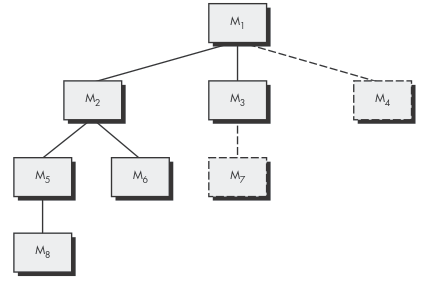
\includegraphics[scale=1]{project/images/profundidad.png}
	\caption{\textbf{Integración descendente}}
\end{figure}
Posteriormente se integrara M6, y finalmente se construyen las rutas de control central (M1-M3-M7) y derecha (M1-M4).\\
La integración primero en anchura incorpora todos los componentes directamente subordinados en cada nivel y se mueve horizontalmente a través de la estructura.\\ Continuando con el ejemplo anterior, los componentes M2-M3-M4 se probarían primero. Después en el siguiente nivel de control M5-M6.
En general, el proceso de integración se realiza en una serie de 5 pasos:
\begin{enumerate}
	\item El módulo de control principal se usa como un controlador de prueba y los representantes (stubs) se sustituyen con todos los componentes directamente subordinados (que son invocados) al módulo de control principal.
	\item Dependiendo del enfoque de integración seleccionado (primero profundidad o primero anchura), los representantes subordinados se sustituyen uno a la vez con componentes reales.
	\item Las pruebas se llevan a cabo conforme se integra cada componente.
	\item Al completar cada conjunto de pruebas, otro representante se sustituye por el componente real.
	\item Las pruebas de regresión pueden realizarse para asegurar que no se introdujeron nuevos errores.
\end{enumerate}
Este proceso se repite desde el paso 2 hasta que se construye toda la estructura del programa.\\
La estrategia de integración descendente verifica los principales puntos de control al principio de cada proceso de prueba. Si se selecciona la integración primero en profundidad, es posible implementar y demostrar el funcionamiento completo del sistema. La integración descendente tiene como complicaciones cuando es necesario que ocurra un procesamiento en los niveles bajos de la jerarquía a fin de probar de manera adecuada los niveles superiores. Ya que al principio de las pruebas, los representantes sustituyen a los módulos de bajo nivel, por lo tanto ningún dato significativo puede fluir hacia arriba en la estructura del programa.\\
Una alternativa para evitar esta problemática resulta en evaluar primero a los módulos con menor jerarquía y posteriormente a los de mayor, a esta estrategia se le conoce como estrategia de integración descendente.\\
\subsubsection{Integración ascendente}
Esta estrategia comienza con la construcción y prueba de módulos atómicos (componentes en los niveles inferiores de la estructura del programa). Puesto que los componentes se integran de abajo hacia arriba, la funcionalidad que proporcionan los componentes subordinados en determinado nivel siempre esta disponible y se elimina la necesidad de representantes.\\
Una estrategia de integración ascendente puede implementarse con los siguientes pasos:
\begin{enumerate}
	\item Los componentes en el nivel inferior se combinan en grupos (llamados construcciones o <<builds>>) que realizan una subfunción de software especifica.
	\item Se escribe un controlador a fin de coordinar la entrada y salida de casos de prueba.
	\item Se prueba el grupo.
	\item Los controladores se remueven y los grupos se combinan moviéndolos hacia arriba en la estructura de programa.
\end{enumerate}
En la figura 2.2 se ejemplifica la integración ascendente. A los módulos de baja jerarquía se les agrupa, en el ejemplo se formaron tres grupos, los cuales están relacionados directamente con un controlador el cual coordinara las entradas y salidas de estos. Los controladores son representados con la letra <<D>> y su respectivo subíndice.\\
Posterior a la realización de las pruebas, los controladores son remplazados por los módulos de jerarquía mayor (en este caso, representados con la letra <<M>>).
\begin{figure}[H]
	\centering
	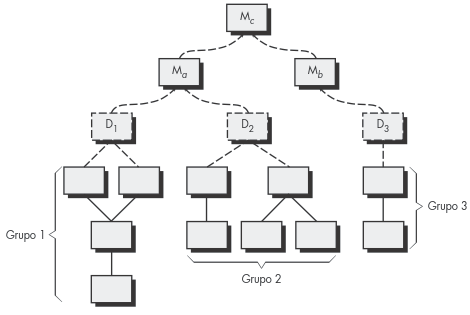
\includegraphics[scale=1]{project/images/integracion.png}
	\caption{\textbf{Integración Ascendente}}
\end{figure}
\subsubsection{Pruebas de regresión}
Cada vez que se agrega un nuevo módulo como parte de las pruebas de integración, el software cambia. Se establecen nuevas rutas de flujo de datos, ocurren nuevas operaciones de entrada o salida y se invoca una nueva lógica de control. Estos cambios pueden causar problemas con las funciones que anteriormente trabajaban sin fallas. En el contexto de una estrategia de pruebas de integración, las pruebas de regresión son la nueva ejecución de algún subconjunto de pruebas que ya se realizaron a fin de asegurar que los nuevos cambios no propagaron efectos no deseados.\\ En general, las pruebas exitosas, dan como resultado el descubrimiento de errores, los cuales son corregidos, cada vez que un error es corregido el software cambia. Las pruebas de regresión ayudan a garantizar que estos cambios no introducen comportamiento no planeado o errores adicionales.\\ Las pruebas de regresión se pueden realizar manualmente o usando herramientas de captura/reproducción, las cuales permiten capturar casos de prueba y resultados para una posterior reproducción y comparación. Las pruebas de regresión se extienden en tres clases diferentes de casos de prueba:
\begin{itemize}
	\item Una muestra representativa de prueba que evaluaran todas las funciones de software.
	\item Pruebas adicionales que se enfocan en las funciones del software que probablemente resulten afectadas por el cambio.
	\item Pruebas que se enfocan en los componentes del software que cambiaron.
\end{itemize}
Conforme avanzan las pruebas de integración, el número de pruebas de regresión puede volverse muy grande, por ende, es necesario que estas sean diseñadas para incluir a una o más clases de errores en cada una de las funciones del programa principal. Resulta impráctico e ineficiente volver a ejecutar todas las pruebas para cada función del programa cada que ocurre un cambio.
\subsubsection{Pruebas de humo}
La prueba de humo consiste en diseñar un mecanismo de ritmo para proyectos críticos en el tiempo, lo que le permite al equipo de software valorar el proyecto de manera frecuente. En general, las pruebas de humo abarcan las siguiente actividades:
\begin{enumerate}
	\item Los componentes se software se integran en una <<construcción>>, la cual incluye todos los archivos de datos, bibliotecas, módulos reutilizables y componentes necesarios que se requieren para implementar una o más funcionalidades del producto.
	\item Se diseña una serie de pruebas para exponer los errores que evitarán a la construcción realizar adecuadamente su función. Esto con la intención de encontrar los errores que puedan retrasar el proyecto.
	\item La construcción, una vez probada, se integra con otras construcciones y el producto (en su forma actual, considerando la cantidad de construcciones integradas) se prueba diariamente. Las construcciones se pueden integrar de manera ascendente o descendente.
\end{enumerate}
Algunas ventajas de implementar las pruebas de humo en un proyecto de software son:
\begin{itemize}
	\item Se minimiza el riesgo de implementación.
	\item La calidad del producto final mejora.
	\item La búsqueda y corrección de errores se simplifica.
	\item El progreso del proyecto es más fácil de valorar.
\end{itemize}
\subsubsection{Integración descendente vs Integración ascendente}
Como se ha analizado anteriormente, ambas estrategias de integración presentan sus respectivas ventajas y desventajas.\\
La selección de una estrategia de integración depende de las características del software y en ocasiones del calendario del proyecto. En general, un enfoque combinado puede resultar en el mejor arreglo.\\ Conforme se avanza en la integración, es necesario identificar los <<módulos críticos>>. Los cuales tienen al menos una de las siguientes características:
\begin{enumerate}
	\item Aborda muchos de los requerimientos del software.
	\item Tiene un alto nivel de control en la estructura del programa.
	\item Es complejo o propenso al error.
	\item Tiene requerimientos de rendimiento definidos.
\end{enumerate}
Estos módulos críticos deben de probarse tanto como sea posible.
\subsubsection{Productos de trabajo de las pruebas de integración}
Un plan global para integración del software y una descripción de las pruebas especificas se documentan en una <<Especificación de pruebas>>. Este producto de trabajo incorpora un plan de prueba y un procedimiento de prueba, y se vuelve parte de la configuración del software. Las pruebas de dividen en fases y construcciones que abordan características del software funcionales y de comportamiento específicas. Cada una de las fases de la prueba de integración delinea una amplia categoría funcional dentro del software y por lo general puede relacionarse con un dominio específico dentro de la arquitectura de software.\\ Los siguiente criterios y pruebas correspondientes se aplican a todas las fases de prueba:
\begin{itemize}
	\item Integridad de la interfaz: Las interfaces internas y externas se prueban conforme cada módulo (o grupo) se incorpora en la estructura.
	\item Validez funcional: Se realizan pruebas diseñadas para descubrir errores funcionales ocultos.
	\item Contenido de la información: Se realizan prueba diseñadas para descubrir errores ocultos asociados con las estructuras de datos locales o globales.
	\item Rendimiento: Se realizan pruebas diseñadas para verificar los limites del rendimiento establecidos durante el diseño de software.
\end{itemize}
En un <<Reporte de pruebas>>, que puede anexarse a la Especificación de pruebas, se registra una historia de resultados, problemas o peculiaridades de prueba reales. Como todos los demás elementos de una configuración de software, el formato de la especificación de pruebas puede adaptarse a las necesidades locales de la organización. Sin embargo, la estrategia de integración y los detalles de las pruebas son esenciales para cualquier especificación.
\subsection{Pruebas de Validación}
\paragraph{Verifican que el software cumpla con los requerimientos especificados.}
Después de la integración del software deben de evaluarse criterios de validación (establecidos durante el análisis de requerimientos).\\ Las pruebas de validación proporcionan la garantía final de que el software cumple con todos los requerimientos informativos, funcionales, de comportamiento y de rendimiento.\\ Se profundiza más en el tema en la sección \textbf{2.5}
\subsection{Pruebas del Sistema}
\paragraph{Verifican la funcionalidad total del sistema.}
El siguiente paso en las pruebas, consiste en que el software una vez validado, debe combinarse con otros elementos del sistema por ejemplo; Hardware, personal, bases de datos, etc.\\ Las pruebas de sistema verifican que todos los elementos se mezclan de una manera adecuada y que se logra el funcionamiento global del sistema.\\ Las pruebas de integración son una técnica sistemática para construir la arquitectura.\\ Se profundiza más en el tema en la sección \textbf{2.6}
\section{Estrategias de Prueba para Software Orientado a Objetos}
El objetivo de probar es encontrar el mayor número posible de errores con una cantidad manejable de esfuerzo aplicado durante un lapso de tiempo realista. A continuación se presentan algunas de las estrategias con las que puede ser probado el software orientado a objetos.
\subsection{Pruebas de unidad en el contexto Orientado a Objetos}
Cuando se considera software orientado a objetos, el concepto de unidad cambia. La encapsulación determina la definición de clases y objetos. Esto significa que cada clase y cada instancia de una clase empaqueta los atributos (datos) y las operaciones que manipulan estos datos.\\ En general, en una clase encapsulada es donde se realizan las pruebas de unidad. Sin embargo, los métodos de estas clases son las las unidades comprobables más pequeñas. Con esto, ya no es posible probar una sola operación en aislamiento sino más bien como parte de una clase.\\
La prueba de clase para software orientado a objetos es el equivalente de la prueba de unidad para software convencional. A las pruebas de clases la dirigen las operaciones encapsuladas por la clase y el comportamiento de estado de ésta.
\subsection{Pruebas de integración en el contexto Orientado a Objetos}
Debido a que como tal no existe una estructura de control jerárquico obvia entre las clases, las estrategias ascendente y descendente difícilmente pueden ser aplicadas. Pero, existen dos estrategias diferentes para realizar la integración.\\
La primera, es la llamada prueba basada en hebra, la cual integra el conjunto de clases requeridas para responder a una entrada o evento del sistema. Cada hebra se integra y prueba de manera individual. Las pruebas de regresión se aplica para asegurar que no ocurran efectos colaterales.\\ El segundo enfoque de integración, son las pruebas basadas en uso, comienzan con la construcción del sistema al probar las llamadas clases independientes. Después de probar las clases independientes, se prueba la siguiente capa de clases, llamadas dependientes, las cuales usan a las clases independientes. Esto se realiza de forma continua hasta que se integra todo el sistema.\\
El uso de controladores y representantes también cambian, los controladores pueden ser usados en un nivel más bajo y para la prueba de todos los grupos de clases, también pueden ser usados para sustituir una interfaz de usuario, de manera que la funcionalidad pueda ser probada antes de la implementación de la interfaz. Los representantes pueden usarse en situaciones donde se requiere la colaboración entre clases pero donde una o más de las clases colaboradoras todavía no se implementa por completo. 
\section{Estrategias de Prueba para Aplicaciones Web}
La estrategia para probar aplicaciones web adopta los principio básicos para todas las pruebas de software y aplica una estrategia y tácticas que se usan para sistemas orientados a objetos. En general puede resumirse en los siguientes pasos:
\begin{enumerate}
	\item El modelo contenido por la aplicación web se revisa para descubrir errores.
	\item El modelo de interfaz se revisa para garantizar que todos los casos de uso pueden adecuarse.
	\item El modelo de diseño para la aplicación web se revisa para descubrir errores de navegación.
	\item La interfaz de usuario se prueba para descubrir errores en los mecanismos de presentación y/o navegación.
	\item A cada componente funcional se le aplica una prueba de unidad.
	\item Se prueba la navegación a lo largo de toda la arquitectura.
	\item La aplicación web se implementa en varias configuraciones ambientales diferentes y se prueba su compatibilidad con cada configuración.
	\item Las pruebas de seguridad se realizan con la intención de explotar vulnerabilidades en la aplicación o en su ambiente.
	\item Se realizan pruebas de rendimiento.
	\item La aplicación se prueba mediante una población de usuarios finales controlada y monitoreada. Los resultados de su interacción con el sistema se evalúan por errores de contenido y de navegación, facilidad de uso, compatibilidad, confiabilidad y rendimiento.
\end{enumerate}
Puesto que muchas aplicaciones web evolucionan constantemente, el proceso de prueba es una actividad que se realiza siempre sobre la marcha, y se realiza para apoyar en las pruebas de regresión derivadas de las pruebas desarrolladas cuando se elaboro por primera vez aplicación web.
\section{Pruebas de Validación}
Las pruebas de validación comienzan en la culminación de las pruebas de integración, cuando ya han sido probados los componentes individuales y ya han sido completamente ensamblados como un paquete y los errores de interfaz se descubrieron y corrigieron. En las pruebas de validación desaparece la distinción entre software convencional, orientado a objetos u aplicaciones web. Las pruebas se enfocan en las acciones visibles para el usuario y las salidas del sistema reconocidas por el usuario.\\
Se pueden decir que la validación es exitosa cuando el software funciona en una forma que cumplas con las expectativas del cliente (lo especificado en el documento de requerimientos de software).
\subsection{Criterios de pruebas de validación}
La validación del software se logra mediante una serie de pruebas que demuestran conformidad con los requerimientos. Un plan de pruebas expresa las clases de pruebas que se van a realizar y un procedimiento de prueba define casos de prueba específicos que se diseñan para garantizar que se satisfagan todos los requerimientos.\\
Después de realizar cada caso de prueba de validación, existen dos posibles condiciones:
\begin{enumerate}
	\item La característica de función o rendimiento se conforma de acuerdo con las especificaciones y se acepta.
	\item Se descubre una desviación de la especificación y se crea una lista de deficiencias. Las cuales rara vez pueden ser corregidas antes de la entrega calendarizada.
\end{enumerate}
Además, es necesario que se tenga una descripción detallada de cada elemento que se desarrollo del software, esto para poder reforzar actividades de apoyo posteriores. A este proceso de revisión comúnmente se le conoce como <<Auditoría>>.
\subsection{Pruebas Alfa y Beta}
En la práctica, es complicado que un desarrollador de software prevea como usará el cliente final el programa. Algunas instrucciones pueden malinterpretarse, algunas salidas para el cliente podrían resultar poco claras para el. Cuando se construye software a la medida, se realizan una serie de pruebas de aceptación a fin de permitir al cliente validar todos los requerimientos. Estas pruebas son realizadas por el usuario final en lugar de un ingeniero de software.\\ Si el software se desarrolla como un producto que será usado por muchos clientes, no es práctico realizar este procedimiento, Para estos casos, son comúnmente usadas las pruebas alfa y beta.\\
\textbf{Las pruebas alfa} se llevan acabo en el sitio del desarrollador por un grupo representativo de usuarios finales El software se usa en el escenario natural con el desarrollador <<a un lado>> de los usuarios registrando errores y problemas de uso. Las pruebas alfa se realizan en un ambiente controlado.\\
\textbf{Las pruebas beta} se realizan en uno o más sitios del usuario final. Donde el desarrollador no se encuentra presente, por lo que las pruebas beta en realidad son la aplicación funcionando <<en vivo>> en un ambiente que no puede controlar el desarrollador. El cliente registra todos los problemas que se encuentre durante la prueba y los reporta al desarrollador periódicamente. Estos errores son corregidos y posteriormente el software vuelve a ser empaquetado y liberado para todos los clientes.
\section{Pruebas del Sistema}
El software, solo es un elemento de un sistema más grande, este debe de incorporarse con otros elementos del sistema, como hardware, personal, información. Para la cual se deben realizar las pruebas de sistema, las cuales son una serie de diferentes pruebas cuyo propósito principal es probar el sistema completo. Aunque cada prueba tenga un propósito diferente, todas funcionan para verificar que los elementos del sistema se hayan integrado de manera adecuada y que realicen las funciones asignadas.
En las siguientes secciones, se mencionan los tipos de prueba del sistema más importantes, como nota, las pruebas de sistema de carga y desempeño, se explican más detalladamente en secciones posteriores. 
\subsection{Pruebas de Recuperación}
La mayoría de los sistemas computacionales, deben de tener la capacidad de recuperarse de fallas y poder reanudar el procesamiento con poco o ningún tiempo de inactividad. A esto se le conoce, como un sistema tolerante a fallas, en los cuales, las fallas en el procesamiento no causan el cese de funcionamiento del sistema global.\\ La recuperación es una prueba del sistema que fuerza al software a fallar en varias formas y verifica que la recuperación se realice de manera adecuada. Si la recuperación es automática (el sistema la realiza en sí), se evalúa el reinicio, los mecanismos de puntos de verificación, la recuperación de datos y la reanudación para las correcciones. Si la recuperación requiere de intervención humana, se evalúa el tiempo medio de reparación para determinar si está dentro de los límites aceptables.
\subsection{Pruebas de Seguridad}
Cualquier sistema que gestione información sensible o cause acciones que puedan dañar (o beneficiar) de manera inadecuada a individuos puede ser blanco de intentos de penetración inadecuada o ilegal.\\
Las pruebas de seguridad, intentan verificar que los mecanismos de protección que se construyen en un sistema en realidad lo protegerán de cualquier intento de penetración ilegal. Durante estas, es necesario que se asuma el papel del individuo que intenta penetrar el sistema y es valido realizar probar con todo tipo de intentos. Por ejemplo, mediante el uso de software hecho a la medida para traspasar las defensas que se hayan construido, intentando abrumar el sistema para así negar el servicio a los demás usuarios, causando errores intencionalmente para intentar penetrar el sistema durante la recuperación, etc.\\ Las buenas pruebas de seguridad al final logran penetrar el sistema, pero se busca, que esta penetración resulte tan costosa (en tiempo y recursos) que sea de mayor valor que la información que se obtendrá del ataque en sí.
\subsection{Pruebas de Despliegue}
En determinados casos, el software debe ejecutarse en varias plataformas y bajo más de un entorno de sistema operativo. Las pruebas de despliegue, en ocasiones llamadas pruebas de configuración, prueban el software en cada entorno en el que este deba operar. Además, examina todos los procedimientos de instalación (esto incluye al software <<instalador>>) que usarán los clientes, así como toda la documentación que se usará para introducir el software a los usuarios finales.\\ En el caso de una aplicación web que funciona bajo el régimen de un navegador, es necesario probar la aplicación web en todos los navegadores sobre los que se piense dar soporte (comúnmente son todos los navegadores modernos) por lo cual aumenta la combinación de pruebas, ya que hay que probar cada navegador web sobre cada sistema operativos hasta cubrir todas las posibilidades (considerando que la compatibilidad entre los mismo lo permita). Las pruebas de seguridad están integradas en cada una de las pruebas de despliegue.
\newpage
\chapter{Pruebas de Usabilidad}
\section{Aspectos Generales}
Al igual que con otros aspectos, es importante probar para validar el nivel de usabilidad que muestra un producto de software.\\ \\

De acuerdo con lo señalado en el estándar ISO/IEC 25010 dentro del cual se identifican características de la calidad del software, la usabilidad se define como “la capacidad de un producto de software para ser entendido, aprendido, utilizado y atractivo hacia el usuario, cuando se usa bajo determinadas condiciones”. Es decir, la usabilidad comprende atributos relacionados con el aprendizaje, la comprensión, la operatividad y lo atractivo del software. \\ \\

Las pruebas de usabilidad se suelen llevar a cabo observando a un grupo de personas mientras usan el producto a probar. Este grupo es seleccionado considerando ciertas características según las condiciones que se desean valorar, según su categoría: usuario experto, medio o inexperto. \\ \\ 

Las métricas de usabilidad suelen ser subjetivas pues requieren de un juicio individual que dependerá de las circunstancias bajo las cuales el producto es usado en su valoración. Sin embargo, existen estándares internacionales, normas y guías de comportamiento respecto a los cuales evaluar, así como métricas que brindan una pauta sobre qué tan “usable” es una aplica.

\section{Clasificación de pruebas de usabilidad}
Las pruebas de usabilidad de clasifican en 3 métodos:
\begin{itemize}
\item Pruebas de usabilidad por inspección
\item Pruebas de usabilidad por indagación
\item Pruebas de usabilidad por test
\end{itemize}

\section{Pruebas de usabilidad por inspección}
El término inspección aplicado a la usabilidad aglutina un conjunto de métodos para probar la usabilidad en los que unos expertos conocidos como evaluadores explican el grado de usabilidad de un sistema basándose en la inspección o examen de la interfaz del mismo. \\ \\
Existen varios métodos que se enmarcan en la clasificación de evaluación por inspección, siendo los siguientes los más importantes:

\subsection{Prueba Heurística}
La “Heurística” es un método de evaluación de sistemas interactivos que consiste en analizar (mediante la inspección de varios evaluadores expertos) la calidad de uso de una interfaz a partir de comprobar su conformidad respecto unos principios reconocidos de usabilidad.
\subsubsection{Modo de aplicación}
Un conjunto de evaluadores expertos en usabilidad contrasta y valida individualmente el conjunto de reglas (o heurísticas, o guidelines) escogido en la interfaz del sistema. Tras las revisiones individuales, los resultados son puestos en común y debatidos en una reunión entre los evaluadores y el responsable de la evaluación, generando el informe final de la evaluación.

\subsection{Recorrido cognitivo}
El recorrido cognitivo (o Cognitive Walkthrough) es un método de inspección de la usabilidad que se centra en evaluar en un diseño su facilidad de aprendizaje, básicamente por exploración y está motivado por la observación que muchos usuarios prefieren aprender software a base de explorar sus posibilidades.
\subsubsection{Modo de aplicación}
Los pasos necesarios para la realización del método son los siguientes:
\begin{enumerate}
	\item Definición de los datos necesarios para el recorrido
	\begin{itemize}
	    \item Se identifican y documentan las características de los usuarios (el tipo de usuario que es dependiendo de su experiencia y el conocimiento adquirido hasta ahora sobre el la aplicación).
	    \item Se describe también el prototipo a utilizar para la evaluación.
	    \item Se enumeran las tareas concretas a desarrollar.
	    \item Para cada tarea se implementa por escrito la lista íntegra de las acciones necesarias para completar la tarea con el prototipo descrito. Esta lista consta de una serie repetitiva de pares de acciones (del usuario) y respuestas (del sistema).
	\end{itemize}
	\item Recorrer las acciones
	\begin{itemize}
	    \item Los evaluadores realizan cada una de las tareas determinadas anteriormente siguiendo los pasos especificados y utilizando el prototipo detallado. En este proceso, el evaluador utilizará la información del usuario (experiencia y conocimiento adquirido) para comprobar si la interfaz es adecuada para el mismo. El evaluador en cada acción criticará el sistema respondiendo a las siguientes preguntas:
	    \begin{itemize}
	        \item ¿Son adecuadas las acciones disponibles de acuerdo a la experiencia y al conocimiento del usuario?
	        \item ¿Percibirán los usuarios que está disponible la acción correcta? Esto se relaciona con la visibilidad y la comprensibilidad de las acciones en la interfaz. 
	        \item Una vez encontrada la acción en la interfaz, ¿asociarán estos usuarios la acción correcta al efecto que se alcanzará?
	        \item Una vez realizada la acción, ¿entenderán los usuarios la realimentación del sistema?
	    \end{itemize}
	\end{itemize}
	\item Documentar los resultados
	\begin{itemize}
	    \item El evaluador anotará para cada acción las respuestas del sistema y sus anotaciones.
	    \item El documento incluirá un anexo especial, conocido como Usability Problem Report Sheet, detallando los aspectos negativos de la evaluación relacionándolos con un grado de severidad que distinga aquellos errores más perjudiciales de los que no lo son tanto. 
	\end{itemize}
\end{enumerate}

\subsection{Recorrido de la usabilidad plural}
Método que comparte algunas características con los recorridos tradicionales pero tiene algunas particularidades que lo diferencian, entre las que cabe destacar la intervención de usuarios finales.
\subsubsection{Modo de aplicación}
Los pasos necesarios para realizar el recorrigo son los siguientes:
\begin{enumerate}
    \item Este método se realiza con tres tipos de participantes, usuarios representativos, desarrolladores y expertos en usabilidad, que conforman todos los actores implicados en el producto.
    \item Las pruebas se realizan con prototipos de papel u otros materiales utilizados en escenarios. Cada participante dispone de una copia del escenario de la tarea con datos que se puedan manipular.
    \item Todos los participantes han de asumir el papel de los usuarios, por tanto, aparte de los usuarios representativos que ya lo son, los desarrolladores y los expertos en usabilidad también lo han de asumir.
    \item Los participantes han de escribir en cada panel del prototipo la acción que tomarán para seguir la tarea que están realizando, escribiendo las respuestas lo más detalladamente posibles.
    \item Una vez que todos los participantes han escrito las acciones que tomarían cuando interactuaban con cada panel, comienza el debate. En primer lugar, deben hablar los usuarios representativos y una vez éstos han expuesto completamente sus opiniones, hablan los desarrolladores y después los expertos en usabilidad.
\end{enumerate}


\subsection{Inspección de estándares}
Para evaluar este método se precisa de un evaluador que sea un experto en los estándares a evaluar. El experto realiza una inspección minuciosa a la interfaz para comprobar que cumple en todo momento y globalmente todos los puntos definidos en el estándar establecido.
\subsubsection{Modo de aplicación}
Si bien este método podría realizarse partiendo de prototipos de baja fidelidad, lo más efectivo es realizarlo a partir de prototipos software o incluso mejor con una primera versión del sistema final donde estén implementadas las partes que deben confrontarse con el estándar (que normalmente serán aspectos más relacionados con la interfaz que con las funcionalidades). \\ \\
En fase de análisis de requisitos se define el estándar que el sistema seguirá (ya sea porque es una especificación del proyecto o uno escogido por sus características) y el experto en dicho estándar realiza una inspección minuciosa a la totalidad de la interfaz para comprobar que cumple en todo momento y globalmente todos los puntos definidos en el estándar. Durante esta exploración, al experto no le importa la funcionalidad de las acciones que va realizando.

\section{Pruebas de usabilidad por indagación}
El proceso de indagación trata de llegar al conocimiento de una cosa discurriendo o por conjeturas y señales. En este tipo de pruebas de la usabilidad una parte muy significativa del trabajo a realizar consiste en hablar con los usuarios y observarlos detenidamente usando el sistema en trabajo real y obteniendo respuestas a preguntas formuladas verbalmente o por escrito. \\ \\
Existen varios métodos que se enmarcan en la clasificación de evaluación por indagación, siendo los siguientes los más importantes.

\subsection{Observación de campo}
La técnica de prueba conocida como Observación de Campo tiene como principal objetivo entender cómo los usuarios de los sistemas interactivos realizan sus tareas y, más concretamente, conocer todas las acciones que realizan durante la ejecución de las mismas. Con ello se pretende capturar toda la actividad relacionada con la tarea y el contexto de su realización así como entender los diferentes modelos mentales que de las mismas tienen los usuarios.
\subsubsection{Modo de aplicación}
La prueba de campo debe prepararse previamente, y esta preparación consiste en:
\begin{itemize}
    \item Escoger una variedad de usuarios representativos del producto.
    \item Utilizar el sitio de observación y el tiempo con eficacia. 
\end{itemize}
Una vez en el lugar, el método se compone básicamente de dos acciones:
\begin{itemize}
    \item La primera y principal es la observación. Observando todo cuanto acontece el lugar de la acción: de qué manera lo hacen, qué botones utilizan, en qué situación los utilizan, dónde buscan las secciones, para qué los utilizan, qué secuencia de acciones siguen, en qué orden lo hacen, cuál es la finalidad, etc.
    \item La segunda y opcional es preguntar o entrevistar. Una vez terminada la observación, se pregunta a los usuarios acerca de su trabajo para complementar la información recabada durante la observación.
\end{itemize}
Al final de una sesión de observación de campo obtendremos una lista de acciones, objetos, personas relacionado con sistema que se está probando.

\subsection{Grupos de discusión o Focus Group}
El Focus Group o Grupo de Discusión es una técnica de recogida de datos donde se reúnen de 6 a 9 personas (generalmente usuarios y también implicados) para discutir aspectos relacionados con el sistema. En ellos un evaluador experto en usabilidad) realiza la función de moderador. Éste preparará previamente la lista de aspectos a discutir y se encargará de recoger la información que necesita de la discusión.
Esto permite capturar reacciones espontáneas e ideas de los usuarios que evolucionan en el proceso dinámico del grupo.
\subsubsection{Modo de aplicación}
El procedimiento general para dirigir un Focus Group es:
\begin{itemize}
    \item Localizar usuarios representativos (típicamente 6 a 9 por sesión) que quieran participar y uno o varios observadores que no intervienen en el debate y sólo toman anotaciones.
    \item Preparar una lista de temas a discutir y los objetivos a asumir por los temas propuestos.
    \item El moderador deberá poner especial énfasis en:
    \begin{itemize}
        \item Que todos los participantes contribuyen a la discusión.
        \item Que no haya un participante que domine la discusión.
        \item Controlar la discusión sin inhibir el flujo libre de ideas y comentarios.
        \item Permitir que la discusión discurra libremente en ciertos momentos pero procurando seguir el esquema planeado.
    \end{itemize}
    \item Al final el moderador (y el/los observador/es) realizará un informe escrito con los resultados y las conclusiones del debate. Incluirá las opiniones que han prevalecido y los comentarios críticos de la sesión.
\end{itemize}

\subsection{Entrevistas}
Una entrevista consiste básicamente en una conversación donde uno o varios usuarios reales del sistema que se va probar o a rediseñar responden a una serie de preguntas relacionadas con el sistema que el entrevistador les va formulando. En este caso, el entrevistador es el evaluador y va tomando nota de las respuestas para obtener las conclusiones finales. \\ \\
Las entrevistas pueden ser estructuradas o abiertas (o desestructuradas), en las primeras el evaluador es más rígido en procurar el buen seguimiento del guión preestablecido, mientras que en las abiertas se da espacio a los implicados a expresarse con más libertad.  \\ \\
Este tipo de evaluación suele realizarse una vez el sistema ya ha sido puesto en marcha, siendo en este caso el principal objetivo captar la satisfacción del cliente o usuario con el producto. El principal problema en estos casos es que si no se ha realizado una correcta planificación de la usabilidad del sistema en ese momento surgen una serie de características que de haber surgido anteriormente se hubieran ahorrado muchos problemas.

\subsection{Cuestionarios}
En el ámbito de prueba de sistemas interactivos hablamos de cuestionarios para referirnos a listas de preguntas que el evaluador distribuye entre usuarios e implicados para que éstos nos las devuelvan respuestas y, así, poder extraer conclusiones. El cuestionario normalmente se distribuye en formato escrito y las preguntas plantean aspectos relacionados con el sistema o aplicación concreta. \\ \\
Así pues, la base del cuestionario es la recolección de información a partir de respuestas contestadas por los usuarios y/o los implicados. \\ \\
Los tipos de preguntas que puede incluir un cuestionario son:
\begin{enumerate}
    \item \textbf{Pregunta de carácter general:} Preguntas que ayudan a establecer el perfil de usuario y su puesto dentro de la población en estudio. 
    \item \textbf{Pregunta abierta:} Preguntas útiles para recoger información general subjetiva. Pueden dar sugerencias interesantes y encontrar errores no previstos.
    \item \textbf{Pregunta de tipo escalar:} Permite preguntar al usuario sobre un punto específico en una escala numérica.   
    \item \textbf{Opción múltiple:} En este caso se ofrecen una serie de opciones y se pide responder a una o varias. Son particularmente útiles para recoger información de la experiencia previa del usuario. Un caso especial es cuando se le dan opciones para contestar si o no.
    \item \textbf{Preguntas ordenadas:} Se presentan una serie de opciones que hay que ordenar.
\end{enumerate}
La actividad de la realización de cuestionarios puede estar ligada a la consecución de ciertas tareas que el evaluador ha creído conveniente realizar (actividad combinada de varios métodos de evaluación) para medir aspectos interactivos del sistema. En estos casos es recomendable dividir el cuestionario en tres partes:
\begin{itemize}
    \item \textbf{Pre-tarea:} Las preguntas de esta sección suelen ser generales acerca de ciertas habilidades del usuario (esta parte suele aprovecharse para recoger información útil acerca del perfil del usuario).
    \item \textbf{Post-tarea:} Esta sección se repetirá tantas veces como tareas tenga que resolver el usuario.
    \item \textbf{Post-test:} Esta sección recogerá aspectos generales acerca de la percepción gomal del usuario tras la consecución de las diferentes tareas planteadas.
\end{itemize}

\section{Pruebas de usabilidad por test}
En los métodos de prueba de usabilidad por test de usuarios representativos se trabaja en tareas utilizando el sistema -o el prototipo- y los evaluadores utilizan los resultados para ver cómo la interfaz de usuario soporta a los usuarios con sus tareas.
Existen varios métodos que se enmarcan en la clasificación de prueba por test, siendo los siguientes los más importantes.

\subsection{Pensando en voz alta (Thinking Aloud) o interacción constructiva}
En este método de evaluación conocido como “thinking aloud” se pide a los usuarios que de forma individual expresen en voz alta y libremente sus pensamientos, sentimientos y opiniones sobre cualquier aspecto (diseño, usabilidad…) mientras que interaccionan con el sistema o un prototipo del mismo. \\ \\
Resulta ser un método altamente eficaz para capturar aspectos relacionados con las actividades cognitivas de los usuarios potenciales del sistema evaluado.
\subsubsection{Modo de aplicación}
Se proporciona a los usuarios el prototipo a probar y un conjunto de tareas a realizar.
\begin{itemize}
    \item Se les pide que realicen las tareas y que expliquen en voz alta qué es lo que piensan al respecto mientras están trabajando con la interfaz, describiendo qué es lo que creen que está pasando, por qué toman una u otra acción o qué es lo que están intentando realizar. 
    \item Pensando en voz alta permite a los evaluadores comprender cómo el usuario se aproxima al objetivo con la interfaz propuesta y qué consideraciones tiene en la mente cuando la usa. El usuario puede expresar que la secuencia de etapas que le dicta el producto para realizar el objetivo de su tarea es diferente de la que esperaba.
\end{itemize}

\subsection{Método del conductor}
El método del conductor es algo diferente a los métodos anteriores en los que hay una interacción explícita entre el usuario y el evaluador (o conductor). \\ \\
Este caso resulta ser totalmente al contrario en este aspecto: Se conduce al usuario en la dirección correcta mientras se usa el sistema. \\ \\
Durante el test, el usuario puede preguntar al evaluador cualquier aspecto relacionado con el sistema y éste le responderá. \\ \\
Este método se centra en el usuario inexperto y el propósito del mismo es descubrir las necesidades de información de los usuarios de tal manera que se proporcione un mejor entrenamiento y documentación al mismo tiempo que un posible rediseño de la interfaz para evitar la necesidad de preguntas.

\subsection{Ordenación de tarjetas (Card Sorting)}
Al comenzar un nuevo ejercicio de diseño de la información es normal encontrarse con una larga lista de ítems sin relacionar que “hay que incluir” y “no sabemos cómo hacerlo”. El reto radica en organizar esta información de manera que sea útil y comprensible para los usuarios del sistema. \\ \\
La técnica conocida como ordenación de tarjetas, o card sorting, es la utilizada para conocer cómo los usuarios visualizan la organización de la información. El diseñador utiliza las aportaciones de los usuarios para decidir cómo deberá estructurarse la información en la interfaz. \\ \\
Se trata de una técnica simple -fácil de entender y de aplicar-, barata, rápida y que involucra a los usuarios, que es especialmente indicada cuando disponemos de una serie de ítems que precisen ser catalogados, así como para decidir la estructura organizativa de cualquier sistema de información. \\ \\
Esta técnica tiene demostrada utilidad para desarrollar sitios web, para la cual está especialmente recomendada.
\subsubsection{Modo de aplicación}
Los pasos a seguir para implementar una ordenación de tarjetas son los siguientes:
\begin{enumerate}
    \item Determinar la lista de tópicos (ítems a ordenar). Esta lista no debería ser muy extensa y comprensible para los participantes de la sesión.
    \item Crear las tarjetas. Cada tópico deberá escribirse en una tarjeta (papel, cartón) que ocasionalmente puede adjuntar algún tipo de explicación. Deberá, además, proporcionar unas cuantas tarjetas en blanco a los participantes.
    \item Seleccionar a los participantes. Los participantes preferentemente serán usuarios finales de quienes deberemos estar seguros que representan fielmente a grupos de usuarios potenciales del sistema.
    \item Proceder con la sesión de ordenación. Cada sesión debe comenzar con una explicación del método y de los objetivos animando a todos los participantes a organizar las tarjetas y etiquetar, en las tarjetas en blanco, los grupos según sus criterios personales. El organizador de la sesión debe tomar nota de todo aquello que pueda resultar relevante para la evaluación final.
    \item Analizar las agrupaciones. Una vez han concluido todos, el evaluador deberá analizar todas las agrupaciones en un ejercicio de “análisis democrático” para identificar aquellas agrupaciones más frecuentes para poder decidir la estructura final.
\end{enumerate}
\newpage
\chapter{Pruebas de Desempeño}
\section{Aspectos Generales}
\noindent
Para sistemas de tiempo real es inaceptable que el software se apegue a la funcionalidad requerida pero sin tomar en cuenta la parte del rendimiento del mismo. Por este motivo existen las pruebas de rendimiento que se diseñan para poner a prueba dicha característica dentro del marco de un sistema integrado. Según Pressman \cite{press} \textit{"Las pruebas de rendimiento requieren de instrumentación de hardware y software"}, podemos interpretar esto como que es necesario medir la utilización de los recursos (memoria, ciclos del procesador, etc) de forma meticulosa.
Las pruebas de rendimiento se usan para descubrir problemas de rendimiento que pueden ser resultado de: falta de recursos, red con ancho de banda o conexión inadecuada, capacidades de base de datos inadecuadas, capacidades de sistema operativo deficientes o débiles, funcionalidad del sistema diseñado y otros conflictos de hardware o software que pueden conducir a un rendimiento degradado. La intención es doble:
\begin{enumerate}
    \item Comprender cómo responde el sistema conforme aumenta la carga(es decir, número de usuarios, número de transacciones o volumen de datos global)
    \item Recopilar mediciones que conducirán a 
modificaciones de diseño para mejorar el rendimiento
\end{enumerate}
\section{Objetivos}
\noindent
Las pruebas de rendimiento se diseñan para simular situaciones de carga del mundo real. Conforme aumenta el número de usuarios simultáneos del sistema el número de transacciones en línea o la cantidad de datos (descargados o subidos), las pruebas de rendimiento ayudarán a responder las siguientes preguntas:
\begin{itemize}
    \item ¿En qué punto (en términos de usuarios, transacciones o carga de datos) el rendimiento 
se vuelve inaceptable?
    \item ¿Qué componentes del sistema son responsables de la degradación del rendimiento?
    \item ¿Cuál es el tiempo de respuesta promedio para los usuarios bajo diversas condiciones de 
carga?
    \item ¿La degradación del rendimiento tiene impacto sobre la seguridad del sistema?
\end{itemize}
Para desarrollar respuestas a estas preguntas, se realizan dos tipos diferentes de pruebas de rendimiento, la prueba de carga examina la carga del mundo real en varios niveles de carga y en varias combinaciones, por otro lado, la prueba de esfuerzo fuerza a aumentar la carga hasta el punto de rompimiento para determinar cuánta capacidad puede manejar el entorno del sistema.
\section{Estrategias de Prueba}
\subsection{Prueba de carga}
\noindent
La intención de la prueba de carga es determinar cómo responderá el sistema y su entorno a varias condiciones de carga. Conforme avanzan las pruebas, las permutas de las siguientes variables definen un conjunto de condiciones de prueba:
\begin{itemize}
    \item \textbf{N} Número de usuarios concurrentes
    \item \textbf{T} Número de transacciones en línea por unidad de tiempo
    \item \textbf{D} Carga de datos procesados por el servidor en cada transacción
\end{itemize}
En todo caso, dichas variables se definen dentro de fronteras operativas normales del sistema. Conforme se aplica cada condición de prueba, se recopila una o más de las siguientes medidas: respuesta de usuario promedio, tiempo promedio para descargar una unidad estandarizada de datos y tiempo promedio para procesar una transacción.\\
La prueba de carga también puede usarse para valorar las velocidades de conexión recomendadas para los usuarios del sistema. El rendimiento global, P, se calcula de la forma siguiente:
\begin{equation}
    P= N * T * D
\end{equation}
\subsection{Prueba de esfuerzo}
\noindent
La prueba de esfuerzo es una continuación de la prueba de carga, pero en esta instancia las variables N, T y D se fuerzan a satisfacerse y luego se superan los límites operativos. La intención de estas pruebas es responder a cada una de las siguientes preguntas:
\begin{itemize}
    \item ¿Las transacciones se pierden conforme la capacidad se excede?
    \item ¿La integridad de los datos resulta afectada conforme la capacidad se excede?
    \item Si el sistema falla, ¿cuánto tiempo tardará en regresar en línea?
    \item ¿Ciertas funciones del sistema quedan descontinuadas conforme la capacidad alcanza el nivel de 80 o 90 por ciento?
\end{itemize}
A una variación de las pruebas de esfuerzo en ocasiones se le conoce como prueba pico/rebote, en este régimen de pruebas, la carga alcanza un pico de capacidad, 
luego se baja rápidamente a condiciones operativas normales y después alcanza de nuevo un pico. Al rebotar la carga del sistema, es posible determinar cuán bien el servidor puede ordenar los recursos para satisfacer una demanda muy alta y entonces liberarlos cuando reaparecen condiciones normales.
\newpage
\chapter{Propuesta Plan de Pruebas}
\section{Propuesta Tipo A}
Instrucciones: En cada etapa que sea concluida es importante que se levante la mano para poder mantener el mismo ritmo en el grupo. Responder la columna de Salidas rellenando el círculo del lado izquierdo con la salida que se obtuvo para terminar o interrumpir la Acción. Seleccionar el error que impidió concluir con la acción.
\subsection*{Etapa 1}
\textbf{Actores:} Alumno, Analista y Académico\newline
\textbf{Prueba:} Iniciar Sesión.
Dirigirse al apartado Iniciar Sesión que se encuentra en la esquina superior derecha de la pantalla principal.
\begin{longtable}{|p{0.7cm}|p{3cm}|p{6cm}|p{2.3cm}|p{3cm}|}
    \hline	
	\textbf{No.}
	&
	\textbf{Entradas}	
	&
	\textbf{Acción}
	&
	\textbf{Salidas}
	&
	\textbf{Error}
	\\
	\hline
	1.
	&
	ID y Contraseña
	&
	1 Ingresar al sistema por medio de los siguientes ID’s correspondientes al tipo de prueba que se fue entregada:\newline
	\textbf{Alumno - Tipo A}\newline
	\textbf{Analista – Tipo B}\newline 
	\textbf{Academico – Tipo C}\newline
	2 Ingresar la siguiente contraseña correspondiente al tipo de prueba que se fue entregada:\newline
	\textbf{aAlumno1 - Tipo A}\newline
	\textbf{bAnalista2 – Tipo B}\newline
	\textbf{cAcademico3 – Tipo C}\newline
	& 	
	O Mensaje de Error\newline
	O Mensaje Positivo\newline
	O Ninguna
	&
	O Contraseña no corresponde\newline
	O ID inexistente\newline
	O Los campos son correctos y los marca como incorrectos\\
	\hline
	2. 
	&
	ID y Contraseña
	&
	1 Repetir el paso uno de la acción anterior.\newline
	2 Ingresar la siguiente contraseña correspondiente al tipo de prueba que se fue entregada:\newline
	\textbf{Alumno1- Tipo A}\newline
	\textbf{Analista2 – Tipo B}\newline
	\textbf{Academico3 -  Tipo C}\newline
	& 	
	O Mensaje de Error\newline
	O Mensaje Positivo\newline
	O Ninguna
	&
	O Contraseña no corresponde
	O ID inexistente 
	O Los campos son correctos y los marca como incorrectos\\
	\hline
\end{longtable}
\section*{Etapa 2}
\textbf{Actores:} Alumno\newline
\textbf{Prueba:} Guardar Horario
Cerrar la sesión (se encuentra en la parte superio derecha de la pantalla) e iniciar sesión con el nuevo usuario (número de boleta y contraseña).\newline
Dirigirse al apartado Reinscripción del menú que se encuentra en la parte izquierda de la pantalla, seleccionar Guardar Horario. 
\begin{longtable}{|p{0.7cm}|p{3cm}|p{6cm}|p{2.3cm}|p{3cm}|}
    \hline	
	\textbf{No.}
	&
	\textbf{Entradas}	
	&
	\textbf{Acción}
	&
	\textbf{Salidas}
	&
	\textbf{Error}
	\\
	\hline
	1.
	&
	Buscar Materia	
	&
	1 Buscar una materia.\newline
	2 Seleccionar la materia con el horario y profesor que se desee.\newline
	3 Repetir el paso 1 y 2 hasta tener 6 materias elegidas.\newline
	4 Seleccionar guardar.	 	
	&
	O Mensaje de Error\newline
 	O Mensaje Positivo\newline
 	O Ninguna
 	&
 	O No existe la materia a buscar y es una materia válida en el mapa curricular.\newline
 	O No agrega la materia.\\
 	\hline
 	2.
 	&
	Buscar Materia	
	&
	1 Buscar la materia: Sistemas Operativos.\newline
	2 Repetir el paso 1 dos veces.
	&
	O Mensaje de Error\newline
 	O Mensaje Positivo\newline
 	O Ninguna
 	&
 	O No existe la materia a buscar.\newline
 	O Los resultados arrojados son distintos en cada búsqueda.\\
	\hline
	3.
	&
	Buscar Materia	
	&
	1 Buscar la materia: Administración de Proyectos. \newline
	2 Agregar 2 veces la materia.
	&
	O Mensaje de Error\newline
 	O Mensaje Positivo\newline
 	O Ninguna
 	&
 	O No existe la materia a buscar.\newline
 	O No agrega la materia.\\
 	\hline
\end{longtable}
\section*{Etapa 3}
\textbf{Actores:} Alumno\newline
\textbf{Prueba:} Revisar Cita de Reinscripción.
Dirigirse al apartado Reinscripción que se encuentra en el menú del lado izquierdo de la pantalla, después seleccionar Cita de Reinscripción.
\begin{longtable}{|p{0.7cm}|p{3cm}|p{6cm}|p{2.3cm}|p{3cm}|}
    \hline	
	\textbf{No.}
	&
	\textbf{Entradas}	
	&
	\textbf{Acción}
	&
	\textbf{Salidas}
	&
	\textbf{Error}
	\\
	\hline
	1.
	&
	Ninguna	
	&
	1 Revisar hora y fecha de la reinscripción.\newline
	2 Reportar sino se tiene cita de reinscripción.
	&
	O Mensaje de Error\newline
 	O Mensaje Positivo\newline
 	O Ninguna
 	&
 	O No se ha asignado una cita para reinscripción.\\
 	\hline
\end{longtable}
\section*{Etapa 4}
\textbf{Actores:} Alumno\newline
\textbf{Prueba:} Reinscribir.\newline
Dirigirse al apartado Renscripción que se encuentra en el menú del lado izquierdo de la pantalla, después seleccionar Cita de Reinscripción.
\begin{longtable}{|p{0.7cm}|p{3cm}|p{6cm}|p{2.3cm}|p{3cm}|}
    \hline	
	\textbf{No.}
	&
	\textbf{Entradas}	
	&
	\textbf{Acción}
	&
	\textbf{Salidas}
	&
	\textbf{Error}
	\\
	\hline
	1.
	&
	Buscar Materia	
	&
	1 Revisar la información que parezca acerca del horario que se guardo en la etapa 2.\newline
	2 Si no aparece alguna información continué con la Acción 2.\newline
	3 Si hay materias que no se hayan podido inscribir eliminé las materias y elija nuevas materias (juntar un total de 6 materias a inscribir).
	&
	O Mensaje de Error\newline
 	O Mensaje Positivo\newline
 	O Ninguna	 	 
 	&
 	O La materia no existe.\newline
 	O No cargo el horario anteriormente guardado.\newline
 	O No agrega la materia que selecciono.\\
 	\hline
 	 & &
	4 Seleccionar Terminar Reinscripción. 
	& &
 	O No permitió que Concluyera su reinscripción.\\
	\hline
 	2.
	&
	Buscar Materia	
	&
	1 Buscar una materia.\newline
	2 Seleccionar la materia para añadir  al futuro horario.\newline
	3 Repetir el punto 1 y 2 seis veces (para juntar un total de seis materias a inscribir).\newline
	4 Seleccionar Terminar Reincripción. 	
	&
	O Mensaje de Error\newline
 	O Mensaje Positivo\newline
 	O Ninguna	 	 
 	&
 	O La materia no existe.\newline
 	O No agrega la materia que selecciono.\newline
 	O No permitió que Concluyera su reinscripción.\\
 	\hline
\end{longtable}
\section*{Etapa 5}
\textbf{Actores:} Alumno\newline
\textbf{Prueba:} Confirmar Horario Inscrito.\newline
Dirigirse al apartado Horario Actual.
\begin{longtable}{|p{0.7cm}|p{3cm}|p{6cm}|p{2.3cm}|p{3cm}|}
	\hline
	\textbf{No.}
	&
	\textbf{Entradas}	
	&
	\textbf{Acción}
	&
	\textbf{Salidas}
	&
	\textbf{Error}
	\\
	\hline
	1.
	&
	Ninguna	
	&
	1 Revisar el horario.\newline
	2 El número de materias inscritas tiene que ser igual a seis en este caso.\newline
	3 Revisar el horario y el profesor.
	&
	O Mensaje de Error\newline
 	O Mensaje Positivo\newline
 	O Ninguna	 	
 	&
 	O No agrego un horario nuevo.\newline
 	O Las materias tienen los datos equivocados.\\
 	\hline
\end{longtable}
\newpage
\section*{Etapa 6}
\textbf{Actores:} Alumno\newline
\textbf{Prueba:} Revisar Cita de Reinscripción.\newline
Dirigirse al apartado Reinscripción que se encuentra en el menú del lado izquierdo.
\begin{longtable}{|p{0.7cm}|p{3cm}|p{6cm}|p{2.3cm}|p{3cm}|}
	\hline
	\textbf{No.}
	&
	\textbf{Entradas}	
	&
	\textbf{Acción}
	&
	\textbf{Salidas}
	&
	\textbf{Error}
	\\
	\hline
	2.
	&
	Ninguna	
	&
	1 Revisar el mensaje que muestra al seleccionar Reinscripción. 	
	&
	O Mensaje de Error\newline
 	O Mensaje Positivo\newline
 	O Ninguna	 	
 	&
 	O Me deja reinscribir más materias\\
 	\hline
\end{longtable}
\newpage
\section{Propuesta Tipo B}
Instrucciones: En cada etapa que sea concluida es importante que se levante la mano para poder mantener el mismo ritmo en el grupo. Responder la columna de Salidas rellenando el círculo del lado izquierdo con la salida que se obtuvo para terminar o interrumpir la Acción. Seleccionar el error que impidió concluir con la acción.
\subsection*{Etapa 1}
\textbf{Actores:} Alumno, Analista y Académico\newline
\textbf{Prueba:} Iniciar Sesión.
Dirigirse al apartado Iniciar Sesión que se encuentra en la esquina superior derecha de la pantalla principal.
\begin{longtable}{|p{0.7cm}|p{3cm}|p{6cm}|p{2.3cm}|p{3cm}|}
    \hline	
	\textbf{No.}
	&
	\textbf{Entradas}	
	&
	\textbf{Acción}
	&
	\textbf{Salidas}
	&
	\textbf{Error}
	\\
	\hline
	1.
	&
	ID y Contraseña
	&
	1 Ingresar al sistema por medio de los siguientes ID’s correspondientes al tipo de prueba que se fue entregada:\newline
	\textbf{Alumno - Tipo A}\newline
	\textbf{Analista – Tipo B}\newline 
	\textbf{Academico – Tipo C}\newline
	2 Ingresar la siguiente contraseña correspondiente al tipo de prueba que se fue entregada:\newline
	\textbf{aAlumno1 - Tipo A}\newline
	\textbf{bAnalista2 – Tipo B}\newline
	\textbf{cAcademico3 – Tipo C}\newline
	& 	
	O Mensaje de Error\newline
	O Mensaje Positivo\newline
	O Ninguna
	&
	O Contraseña no corresponde\newline
	O ID inexistente\newline
	O Los campos son correctos y los marca como incorrectos\\
	\hline
	2. 
	&
	ID y Contraseña
	&
	1 Repetir el paso uno de la acción anterior.\newline
	2 Ingresar la siguiente contraseña correspondiente al tipo de prueba que se fue entregada:\newline
	\textbf{Alumno1- Tipo A}\newline
	\textbf{Analista2 – Tipo B}\newline
	\textbf{Academico3 -  Tipo C}\newline
	& 	
	O Mensaje de Error\newline
	O Mensaje Positivo\newline
	O Ninguna
	&
	O Contraseña no corresponde.\newline
	O ID inexistente.\newline
	O Los campos son correctos y los marca como incorrectos.\\
	\hline
\end{longtable}
\newpage
\section*{Etapa 2}
\textbf{Actores:} Analista\newline
\textbf{Prueba:} Registrar Alumno.\newline
Dirigirse al apartado Registro que se encuentra en el menú del lado izquierdo de la pantalla, después seleccionar Registrar Alumno.
\begin{longtable}{|p{0.7cm}|p{3cm}|p{6cm}|p{2.3cm}|p{3cm}|}
    \hline	
	\textbf{No.}
	&
	\textbf{Entradas}	
	&
	\textbf{Acción}
	&
	\textbf{Salidas}
	&
	\textbf{Error}
	\\
	\hline
	1.
	&
	Nombre\newline
	Apellidos\newline
	Correo electrónico\newline
	Contraseña\newline
	Contraseña (confirmación)	
	&
	1. Llenar los campos que solicitan con la información de su compañero de alado como alumno (el correo electrónico debe ser existente). La contraseña debe ser asignada por usted utilizando la primera letra del nombre y el primer apellido, ejemplo:\newline
	Nombre: América Monsalvo.\newline
	Contraseña: amonsalvo.	 	
	&
	O Mensaje de Error\newline
 	O Mensaje Positivo\newline
 	O Ninguna	 	
 	&
 	O El alumno ya ha sido registrado.\newline
 	O Los campos son correctos y los marca como incorrectos.\\
 	\hline
\end{longtable}
\section*{Etapa 3}
\textbf{Actores:} Analista\newline
\textbf{Prueba:} Generar Cita.\newline
Dirigirse al apartado Periodos que se encuentra en el menú del lado izquierdo de la pantalla, después seleccionar Generar Cita.
\begin{longtable}{|p{0.7cm}|p{3cm}|p{6cm}|p{2.3cm}|p{3cm}|}
    \hline	
	\textbf{No.}
	&
	\textbf{Entradas}	
	&
	\textbf{Acción}
	&
	\textbf{Salidas}
	&
	\textbf{Error}
	\\
    \hline
	1.
	&
	Fecha Inicio\newline
	Fecha Termino\newline
	Hora inicio\newline
	Hora termino\newline
	Tiempo de  reinscripción	
	&
	1 Selección como fecha de inicio el día en que se está ejerciendo la prueba.\newline
	2 Seleccionar como fecha de termino los tres días hábiles posteriores a la fecha de inicio.\newline
	3 Seleccionar Hora de inicio  las 8 a.m. y hora de término las 4 p.m.	 	
	&
	O Mensaje de Error\newline
 	O Mensaje Positivo\newline
 	O Ninguna	 	 
	&
 	O Ya existe un periodo de inscripción.\newline
 	O El rango de horas no está permitido.\newline
 	O Las fechas no son días hábiles.\newline
 	O El tiempo de reinscripción no es suficiente.\\
 	\hline
 	  & &
 	3 Seleccionar el Tiempo de reinscripción de 30 minutos.\newline
	4 Seleccionar Aceptar.
	& &
 	O Los campos son válidos y los marca como incorrectos.\\
 	\hline
\end{longtable}
\section*{Etapa 4}
\textbf{Actores:} Analista\newline
\textbf{Prueba:} Reinscribir\newline
Dirigirse al apartado Renscribir que se encuentra en el menú del lado izquierdo de la pantalla, después seleccionar Reinscripción.
\begin{longtable}{|p{0.7cm}|p{3cm}|p{6cm}|p{2.3cm}|p{3cm}|}
    \hline	
	\textbf{No.}
	&
	\textbf{Entradas}	
	&
	\textbf{Acción}
	&
	\textbf{Salidas}
	&
	\textbf{Error}
	\\
    \hline
	1.
	&
	Buscar Materia\newline
	Buscar Alumno	
	&
	1 Seleccionar el alumno que se desea inscribir.\newline
	2 Buscar Materia que el alumno solicité a inscribir.\newline
	3 Seleccionar Materia.\newline
	4 Repetir los pasos 2 y3 seis veces para juntar un total de seis materias a inscribir. Si la materia no puede ser inscrita utilicen otra materia.\newline
	5 Seleccionar Terminar reinscripción.
	&
	O Mensaje de Error\newline
 	O Mensaje Positivo\newline
 	O Ninguna	 	 
	&
 	O La materia no existe.\newline
 	O No agrega la materia que selecciono.\newline
 	O No permitió que Concluyera su reinscripción.\\
 	\hline
\end{longtable}
\newpage
\section{Propuesta Tipo C}
Instrucciones: En cada etapa que sea concluida es importante que se levante la mano para poder mantener el mismo ritmo en el grupo. Responder la columna de Salidas rellenando el círculo del lado izquierdo con la salida que se obtuvo para terminar o interrumpir la Acción. Seleccionar el error que impidió concluir con la acción.
\subsection*{Etapa 1}
\textbf{Actores:} Alumno, Analista y Académico\newline
\textbf{Prueba:} Iniciar Sesión.
Dirigirse al apartado Iniciar Sesión que se encuentra en la esquina superior derecha de la pantalla principal.
\begin{longtable}{|p{0.7cm}|p{3cm}|p{6cm}|p{2.3cm}|p{3cm}|}
    \hline	
	\textbf{No.}
	&
	\textbf{Entradas}	
	&
	\textbf{Acción}
	&
	\textbf{Salidas}
	&
	\textbf{Error}
	\\
	\hline
	1.
	&
	ID y Contraseña
	&
	1 Ingresar al sistema por medio de los siguientes ID’s correspondientes al tipo de prueba que se fue entregada:\newline
	\textbf{Alumno - Tipo A}\newline
	\textbf{Analista – Tipo B}\newline 
	\textbf{Academico – Tipo C}\newline
	2 Ingresar la siguiente contraseña correspondiente al tipo de prueba que se fue entregada:\newline
	\textbf{aAlumno1 - Tipo A}\newline
	\textbf{bAnalista2 – Tipo B}\newline
	\textbf{cAcademico3 – Tipo C}\newline
	& 	
	O Mensaje de Error\newline
	O Mensaje Positivo\newline
	O Ninguna
	&
	O Contraseña no corresponde\newline
	O ID inexistente\newline
	O Los campos son correctos y los marca como incorrectos\\
	\hline
	2. 
	&
	ID y Contraseña
	&
	1 Repetir el paso uno de la acción anterior.\newline
	2 Ingresar la siguiente contraseña correspondiente al tipo de prueba que se fue entregada:\newline
	\textbf{Alumno1- Tipo A}\newline
	\textbf{Analista2 – Tipo B}\newline
	\textbf{Academico3 -  Tipo C}\newline
	& 	
	O Mensaje de Error\newline
	O Mensaje Positivo\newline
	O Ninguna
	&
	O Contraseña no corresponde
	O ID inexistente 
	O Los campos son correctos y los marca como incorrectos\\
	\hline
\end{longtable}
\section*{Etapa 2}
\textbf{Actores:} Académico\newline
\textbf{Prueba:} Registrar Horario.\newline
Dirigirse al apartado Administrar que se encuentra en el menú del lado izquierdo de la pantalla, después seleccionar Registrar Horario.
\begin{longtable}{|p{0.7cm}|p{3cm}|p{6cm}|p{2.3cm}|p{3cm}|}
    \hline	
	\textbf{No.}
	&
	\textbf{Entradas}	
	&
	\textbf{Acción}
	&
	\textbf{Salidas}
	&
	\textbf{Error}
	\\
	\hline
	1.
	&
	Materia\newline
	Profesor\newline
	Grupo\newline
	Hora	
	&
	1 Seleccionar la Materia: Compiladores.\newline
	2 Seleccionar la Materia: Administración Financiera.
	&
	O Mensaje de Error\newline
 	O Mensaje Positivo\newline
 	O Ninguna	 	
 	&
 	O La materia no existe.\newline
 	O No actualiza los profesores que imparten la materia.\\
 	\hline
 	2.
	&
	Materia\newline
	Profesor\newline
	Grupo\newline
	Horario	
	&
	1 Seleccionar la Materia: Bases de Datos.\newline
	2 Seleccionar al primer profesor que aparezca.\newline
	3 Seleccionar el Grupo (el tercer grupo en aparecer).\newline
	4 Seleccionar el Horario.\newline
	5 Seleccionar Registrar.
	&
	O Mensaje de Error\newline
 	O Mensaje Positivo\newline
 	O Ninguna	 	
 	&
 	O La materia no existe.\newline
 	O No actualiza los profesores que imparten la materia.\newline
 	O La materia ya ha sido registrada en el grupo.\newline
 	O El horario ya ha sido ocupado por otra materia.\\
 	\hline
 	3.
	&
	Materia\newline
	Profesor\newline
	Grupo\newline
	Horario	
	&
	1 Seleccionar alguna Materia.\newline
	2 Seleccionar al primer profesor que aparezca.\newline
	3 Seleccionar el Grupo.\newline
	4 Seleccionar el Horario.\newline
	5 Seleccionar Registrar.\newline
	6 Si la materia ya ha sido registrada o el horario está ocupado intentar con otra materia, o cambiar algún campo que permita registrar la materia. Después de 5 intentos fallidos  concluya esta Etapa.
	&
	O Mensaje de Error\newline
 	O Mensaje Positivo\newline
 	O Ninguna	 	
 	&
 	La materia no existe.\newline
 	No actualiza los profesores que imparten la materia.\newline
 	No registro la materia en 5 intentos.\newline
 	La materia no tiene disponibilidad de horario.\\
 	\hline
\end{longtable}
\section*{Etapa 3}
\textbf{Actores:} Académico\newline
\textbf{Prueba:} Editar Horario.\newline
Dirigirse al apartado Administrar que se encuentra en el menú del lado izquierdo de la pantalla, después seleccionar Editar Horario.
\begin{longtable}{|p{0.7cm}|p{3cm}|p{6cm}|p{2.3cm}|p{3cm}|}
    \hline	
	\textbf{No.}
	&
	\textbf{Entradas}	
	&
	\textbf{Acción}
	&
	\textbf{Salidas}
	&
	\textbf{Error}
	\\
    \hline	
	1.
	&
	Buscar Materia\newline
	Materia\newline
	Profesor\newline
	Grupo\newline
	Hora	
	&
	1 Buscar la materia que fue registrada en la Etapa 2.\newline
	2 Modificar al profesor por el segundo que parece.\newline
	3 Seleccionar Guardar.\newline
	4 Si la materia ya ha sido registrada o el horario está ocupado intentar con otro Profesor. Después de 5 intentos fallidos concluya esta Etapa.	 	
	&
	O Mensaje de Error\newline
 	O Mensaje Positivo\newline
 	O Ninguna	 	
 	&
 	O La materia no existe.\newline
 	O No actualiza los profesores que imparten la materia.\newline 
 	O La materia editada no puede ser registrada ya que no tiene disponibilidad de horario.\\
	\hline
\end{longtable}
\newpage
\subsection{Propuesta Cuestionario}
\begin{longtable}{p{15cm} p{1cm}}
    1. Del 0 al 10 (considerando que 0 es no me gusto y 10 es me encanto) ¿Cuánto le agradaron los colores que tiene el sistema SAES?
    &
    [  ]\\
    2. Si la respuesta anterior fue menor o igual a 7, elija el color base que le agradaría que tuviera el sistema SAES (considerando al blanco como su color acompañante), sino pase a la siguiente pregunta.\newline
    a. Guinda  \hspace{2cm} b. Negro  \hspace{2cm} c. Naranja oscuro
    &
    [  ]\\
    3. Del 0 al 5 (considerando 0 como no se puede ver y 5 se ve claramente)¿Qué tan claro podía leer el texto dentro del sistema SAES?
    &
    [  ]\\
    4. ¿El tipo de letra es legible y entendible?\newline
    a. SI   \hspace{2cm} b. NO
    &
    [  ]\\
    5. ¿Los mensajes mostrados por el sistema SAES fueron poco entendibles, ambigüos o poseen faltas de ortografía? \newline
    a. SI \hspace{2cm}  b.NO
    &
    [  ]\\
    6. ¿EL texto en los mensajes, botones, etiquetas y alertas del sistema SAES lo incomodarón, molestarón o irritarón? \newline
    a. SI \hspace{2cm}  b. NO
    &
    [  ]\\
    7. Del 0 a 5 ¿Cómo le parece la velocidad del sistema SAES?  & [  ]\\
    8. Del 0 al 10 ¿Qué le parece la opción de crear un horario y guardarlo? & [  ]\\
    9. Del 0 al 5 ¿Qué le pareció la distribución de las funciones en el menú? & [  ]\\
    10. ¿Recomendaría y/ o usaría el sistema SAES? \newline a. SI \hspace{2cm} b.NO &  [  ]\\ 
\end{longtable}
\vspace*{2cm}
\noindent
Es importante escuchar su opinión por lo que si tiene algún comentario acerca del sistema, le pedimos que lo escribe en las siguientes líneas.
\begin{longtable}{ |p{15cm}| }
\hline
    \vspace*{5cm} \\
\hline
\end{longtable}
%\newpage
\addcontentsline{toc}{chapter}{Referencias Bibliográficas}
\begin{thebibliography}{99}
\bibitem{IN1} CapItulo 20. Protocolo SSH. (n.d.). Retrieved May 19, 2019, from https://web.mit.edu/rhel-doc/4/RH-DOCS/rhel-rg-es-4/ch-ssh.html
\bibitem{IN1} HTTP. (n.d.). Retrieved May 19, 2019, from https://developer.mozilla.org/es/docs/Web/HTTPReferencias
\bibitem{IN1} Protocolo de transferencia de archivos. (2019, May 06). Retrieved May 19, 2019, from https://es.wikipedia.org/wiki/Protocolo-de-transferencia-de-archivos
\bibitem{IN1} ¿Qué es DNS? – Introducción a DNS - AWS. (n.d.). Retrieved May 19, 2019, from https://aws.amazon.com/es/route53/what-is-dns/
\bibitem{IN1} ¿Qué es un Servidor SMTP? Qué significa y cómo usarlo para enviar email. (2019, January 09). Retrieved May 19, 2019, from https://es.mailjet.com/blog/news/servidor-smtp/
\end{thebibliography}
\end{comment}
\end{document}